%% Outline

%%%% Intro
% Objetivido do sistema
% Importnacia
% É o que a Amazon usa e foram eles que inventaram

%%%%% Arquitetura
% 0. Sistema como u todo
% Imgens
% 1. API
% O que faz 
% 2. KVS LOcal
% O que faz 
% 3.  
% O que faz 

%%%%% Implementação
% 1. API
% O que faz 
% O que contem (modulos, ficheiros, funcoes)
% o que guarda (estruturas)
% Thread management

% 2. KVS LOcal
% O que faz 
% O que contem (modulos, ficheiros, funcoes)
% o que guarda (estruturas)
% Thread management
% delete group
% groups in multiple KVS locals

%%%%%%%%% Communication
% 1. API - KVS LOcal 
% sockets properties (reliability)
% protocolo
% limites

% 2. Callbacks
% sockets properties (reliability)
% protocolo
% limites

% 3. KVS Local - Auth
% sockets properties (message oriented)
% How is managed the nondelivery guarantees oft he datagramsockets
% protocolo
% limites

%% 4. Sequence diagrams

%%&%%%%% Paralellemmism [Leo]
% 1. Synch

%%%%% Validation 
% testes que fizemos
% transferencia de ficheiro grande 
% transferencia de imagem 

\section{Introdução}

%%%% Intro
% Objetivo do do sistema
% Importancia
% É o que a Amazon usa e foram eles que inventaram

No âmbito da Unidade Curricular de Programação de Sistemas, desenvolveu-se o presente relatório acerca do projeto focado no desenvolvimento de uma Key-Value Store. De acordo com \cite{amazon}, este sistema é um tipo de base de dados não relacional (por oposição a bases de dados relacionais que se baseiam no conceito de tabelas) utilizada por empresas como a Amazon em que os dados são acedidos apenas com uma chave e tanto os dados como a chave podem tomar qualquer valor. Este sistema tem como vantagem a capacidade de escalar grandes quantidades de dados com muitas modificações enquanto serve bastantes clientes.

No que toca ao relatório, este pretende mostrar como se interpretou o sistema, explicar detalhadamente a implementação desenvolvida, e justificar as decisões tomadas. Em primeiro lugar, discute-se o sistema no seu todo e as funcionalidades necessárias em cada um dos subsistemas. Em segundo lugar, abordam-se os diferentes aspetos da implementação desenvolvida para cada um dos subsistemas, abordando a divisão em ficheiros e funções e as estruturas de dados utilizadas. Em terceiro lugar, explicam-se o funcionamento, as propriedades, e as estruturas de dados dos mecanismos de comunicação entre subsistemas. São ainda apresentadas as sequências de interações realizadas para executar as diferentes funcionalidades do sistema. Por último, apresentam-se as formas de sincronização implementadas nos diversos subsistemas. As diversas decisões de programação tomadas são explicadas à medida que se abordam os temas com elas relacionados.

\section{Arquitetura}\label{sec:Arq}

%%%%% Arquitetura
% 0. Sistema como u todo
% Imgens
% 1. API
% O que faz 
% 2. KVS LOcal
% O que faz 
% 3.  
% O que faz 

Na versão de Key-Value Store a implementar neste projeto, é fornecida a várias aplicações diferentes uma Application Programming Interface (API), desginada por KVS-Lib, que permite a criação e o acesso a pares chaves-valores armazenados num servidor local (local por ser na mesma máquina), KVS-LocalServer. As aplicações constituem assim os primeiros subsistemas do sistema total e os KVS-LocalServers os segundos. As aplicações comunicam com os KVS-LocalServers através de UNIX stream sockets e o servidor local, para gerir os acessos à sua base de dados, exige a autenticação das aplicações por segredos. Os pares, neste subsistema, estão divididos em grupos, pelo que uma aplicação cria e acede a pares num grupo. Por outro lado, como uma aplicação acede a todos os pares num mesmo grupo, a cada segredo corresponde um grupo. Os segredos estão guardados num servidor que pode estar noutra máquina com o qual se comunica através de INET datagram sockets e que se designa por KVS-AuthServer. Este é o terceiro subsistema do sistema total. Podem existir várias aplicações ligadas a um único KVS-LocalServer e vários KVS-LocalServers ligados a um único KVS-AuthServer. Na Fig. \ref{fig:architecture}, ilustra-se a arquitetura anterior. Nas secções seguintes, as funcionalidades dos diversos subsistemas são analisadas com maior detalhe.

\begin{figure}[ht]
    \centering
    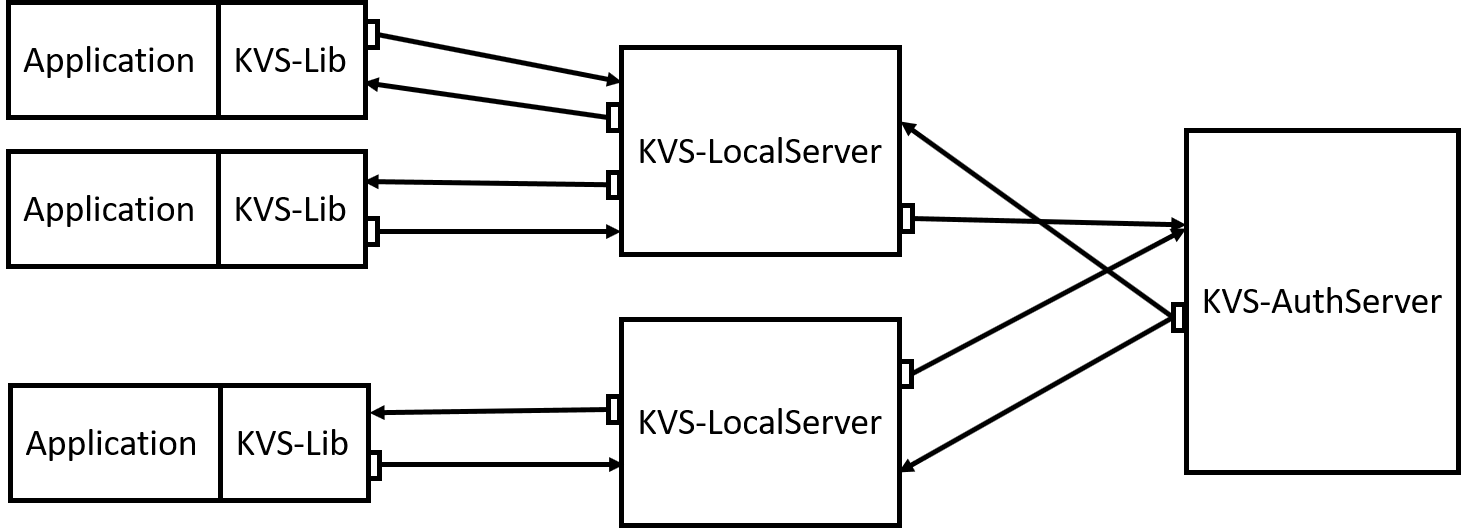
\includegraphics[width=0.7\linewidth]{figures/architecture.png}
    \caption{Arquitetura do sistema completo.}
    \label{fig:architecture}
\end{figure}

\subsection{KVS-Lib} \label{sec:ArqLib}

A KVS-Lib é uma API que deve permitir a uma aplicação as seguintes funcionalidades: i) criar pares de chaves-valores no grupo a que tem acesso; ii) apagar pares de chaves-valores no grupo a que tem acesso; iii) conhecer os valores associados às chaves do grupo a que tem acesso; iv) estabelecer conjuntos de ações que devem ser efetuados quando existe alteração de determinados pares. Para evitar a constante autenticação num grupo, a KVS-Lib deve ainda ter como funcionalidades: v) estabelecer a ligação com um grupo do KVS-LocalServer, o que equivale a iniciar uma sessão em que continuamente pode interagir com esse grupo; vi) fechar a ligação com um grupo do KVS-LocalServer, o que equivale a terminar a anterior sessão, sendo, à parte de falhas, a única forma de terminar a sessão. Por outro lado, a arquitetura utilizada entre a KVS-Lib e o KVS-LocalServer deve ser uma arquitetura de cliente-servidor em que a comunicação, como já foi dito anteriormente, deverá ser realizada através de UNIX stream sockets.

\subsection{KVS-LocalServer}\label{sec:arq_KVSLocal}

O KVS-LocalServer deverá ser executado na mesma máquina que as aplicações que lhe acedem, comunicando com elas por UNIX stream sockets, como já mencionado. Este servidor deverá ter como funcionalidades: i) receber os pedidos de cada cliente através da API; ii) responder a esses pedidos; iii) processar os pedidos de cada cliente; iv) guardar informação da ligação com cada cliente; v) manter uma UI; v); permitir a criação de grupos; vi) permitir a eliminação de grupos; vii) apresentar a informação referente a cada grupo; viii) apresentar a informação referente a cada cliente; ix) armazenar os grupos de pares; x) obter segredos do KVS-AuthServer; xi) autenticar clientes; xii) comunicar alterações sobre os grupos ao KVS-AuthServer; xiii) alertar os clientes da alteração de pares com que eles estabeleceram conjuntos de ações a serem executadas. Este servidor deve comunicar com um KVS-AuthServer através de INET datagram sockets, como já referido, numa arquitetura cliente-servidor.

\subsection{KVS-AuthServer} \label{sec:arch_auth}

O KVS-AuthServer pode ser executado numa máquina diferente e comunica com os KVS-LocalServers através de INET datagram sockets numa arquitetura cliente-servidor, como já referido. Este servidor deverá ter como funcionalidades: i) receber os pedidos de cada KVS-LocalServer; ii) processar esses pedidos; iv) armazenar os pares de grupos e segredos.

\section{Implementação}

% 0. Sistema como u todo
% Imagens

A arquitetura dos anteriores subsistemas é implementada em linguagem C de acordo com o explicado nesta secção. A comunicação entre subsistemas é realizada tal como explicado na Secção \ref{sec:com}. É de salientar que na implementação do sistema se procurou utilizar o princípio \textit{Least knowledge} entre subsistemas e que em todas as funções ou módulos não se sobrecarregasse as suas funcionalidades.

Por outro lado, procurou-se compartimentar as funcionalidades em módulos correspondentes a ficheiros \texttt{.c} e correspondentes \texttt{.h} no código. Estes ficheiros interagem entre si dentro do mesmo subsistema e podem ser observados no diagrama da Fig. \ref{fig:architecture_detail} de acordo com o seu nível de abstração. É de notar que se desenvolveu os subsistemas de forma a que pudessem ser independentemente compilados e transferidos entre máquinas com ficheiros \texttt{Makefile} individuais.

\begin{figure}[ht!]
    \centering
    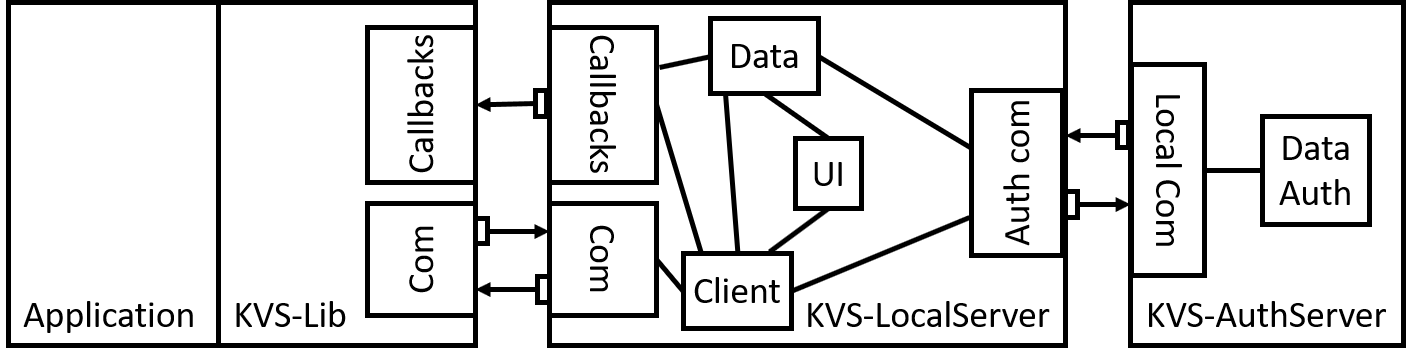
\includegraphics[width=0.7\linewidth]{figures/architecture_detail.png}
    \caption{Arquitetura implementada do sistema completo.}
    \label{fig:architecture_detail}
\end{figure}

\subsection{KVS-Lib API}
% 1. API
% O que faz 
% O que contem (modulos, ficheiros, funcoes)
% o que guarda (estruturas)
% Thread management
As funcionalidades descritas na Secção \ref{sec:ArqLib} são implementadas através do conjunto de funções da KVS-Lib API na Listing \ref{lstprot}, cujo nome é indicativo da sua funcionalidade.
\begin{lstlisting}[language=C,label={lstprot},caption=Protótipos da KVS-Lib API.]
int establish_connection (char * group_id, char * secret);
int put_value(char * key, char * value);
int get_value(char * key, char ** value);
int delete_value(char * key);
int register_callback(char * key, void (*callback_function)(char *));
int close_connection();
\end{lstlisting}

Nesta subsecção é descrita a forma como cada uma destas funcionalidades é implementada de acordo com a arquitetura servidor-cliente proposta na Secção \ref{sec:Arq}. O ficheiro principal que o implementa e interage com as implementações dos restantes componentes designa-se \texttt{KVS-lib.c}. De forma a estruturar esta implementação, foi dividida em três grandes partes: 
\begin{enumerate}[noitemsep]
    \item  Pedidos e respostas de informação do KVS-LocalServer (\say{com} na Fig. \ref{fig:architecture_detail}), implementado no ficheiro \texttt{KVSlib-com.c} e no respetivo \textit{header file}.
    \item Deteção e registo de callbacks (\say{Callbacks} na Fig. \ref{fig:architecture_detail}), implementado no ficheiro \texttt{KVSlib-cb.c} e no respetivo \textit{header file}.
\end{enumerate}
Para além dos \textit{header files} associados a cada um dos ficheiros \texttt{.c}, existe a necessidade de incluir \textit{headers} adicionais com macros e estruturas de dados que têm de ser partilhadas entre módulos do KVS-LocalServer, ou mesmo entre subsistemas. Assim, foram adicionados os seguintes headers:
\begin{enumerate}[noitemsep]
 \item \texttt{KVS-lib-MACROS.h} é comum a todos os subsistemas e permite concordar nos tamanhos máximos das strings \texttt{groupId} e \texttt{secret};
\item \texttt{KVSLocalServer-base.h} é comum a todos os módulos a KVS-Lib e permite a inclusão de bibliotecas C para implementar as funcionalidades desejadas;
\item \texttt{KVS\_local-lib\_com.h} é partilhado entre os módulos de comunicação mútua da KVS-Lib e do KVS-LocalServer, de forma a poder acordar em identificadores de mensagens e valores de retorno distintos no caso de um erro.
\end{enumerate}

O conjunto de ficheiros do source code da KVS-Lib API foi agregado num ficheiro \textit{archive} (com extensão \texttt{.a}). Assim, pode ser incluído de forma estática numa aplicação em conjunto com um único \textit{header file} da API \texttt{KVS-lib.h}. É de notar foi gerado um \textit{archive} ao invés de um \textit{shared object} (com extnsão \texttt{.so}), ainda que os último sejam mais usado atualmente. No entanto, visto não se considerar ser necessário incluir a API numa aplicação de forma dinâmica, durante a sua execução, e que a criação de um \textit{archive} é mais fácil, optou-se por esta opção.

%%%%%%Criamos a partir da kvs lob o .c no ponto a archive. Explicar que o ponto a juntamente com o ponto h pode ser utilizado em vários sistemas operativos unix sendo facilemnet compilado com o clinet e

\subsubsection{Pedidos e respostas de informação do KVS-LocalServer}
Em primeiro lugar, serão detalhados os pedidos e respostas que será necessário trocar com o KVS-LocalServer de forma a implementar as funcionalidades descritas. O canal de comunicação usado serão UNIX domain stream sockets, que permitem a troca bidirecional de informação. A forma como esta informação é trocada e o protocolo de comunicação usado nesta interface são detalhados na Secção \ref{com:lib_local}.

Assim, é necessário definir, para cada uma das funções da API, quais os argumentos do pedido (query) e quais os argumentos da resposta (response) que se espera receber.  Na Tabela \ref{tab:args_query_resp} são apresentados os argumentos da query feita em cada uma das funções e os argumentos que se espera receber como resposta. Note-se que em cada pedido efetuado ao KVS-LocalServer é recebido um status, que permite saber se a operação foi concluída com sucesso e, caso contrário, qual o erro que se verificou. Os erros identificados no KVS-LocalServer, KVS-AuthServer, e na própria API são retornados para o utilizador na função em que o erro ocorreu. O conjunto de output status disponíveis para o utilizador verificar o status da função executada é apresentado na Tabela \ref{tab:status_val}.

\begin{table}[ht!]
    \centering
     \caption{Conteúdos das mensagens trocadas entre KVS-Lib e KVS-LocalServer.}
    \begin{tabular}{ccc}
    \hline
         Função &  Query args & Response args\\
         \hline
         \texttt{establish\_connection} & PID, \texttt{groupId}, \texttt{seret} & status \\
         \texttt{put\_value} & \texttt{key}, \texttt{value} & status\\
         \texttt{get\_value} & \texttt{key} & status, \texttt{value} \\
         \texttt{delete\_value} & \texttt{key} & status \\
         \texttt{register\_callback} & \texttt{key}, \texttt{cb\_id} & status \\
         \texttt{close\_connection} & -- & status \\
         \hline
    \end{tabular}
   
    \label{tab:args_query_resp}
\end{table}


\begin{table}[ht!]
    \centering
     \caption{Output status.}
    \begin{tabular}{ll}
        \hline
         status & Description\\  
         \hline
         \texttt{SUCCESS} & Completado com sucesso.\\
         \texttt{ERROR\_ACCSS\_DENIED} & Acesso negado, ação não autorizada. \\
         \texttt{ERROR\_GROUP\_DSNT\_EXIST} & O grupo indicado não existe. \\
         \texttt{ERROR\_ALLOC} & Erro de alocação de memória. \\
         \texttt{ERROR\_KEY\_DSNT\_EXIST} & A \texttt{key} indicada não existe. \\
         \texttt{ERROR\_INVALID\_ARG\_LEN} & O tamanho dos argumentos é inválido. \\
         \texttt{ERROR\_CREATING\_SOCK} & Erro na criação da socket de comunicação com o KVS-LocalServer. \\
         \texttt{ERROR\_CONNECTION\_SERVER} & Erro na conexão à socket do KVS-LocalServer.  \\
         \texttt{ERROR\_COM\_SERVER} & Erro na comunicação com o KVS-LocalServer. \\
         \texttt{ERROR\_DISCONNECTED\_SOCK} & A socket de comunicação com o KVS-LocalServer está disconectada. \\
         \texttt{ERROR\_CALLBACK\_SOCK} & Erro na criação, bind, ou listen da socket dos callbacks.\\
         \texttt{ERROR\_CALLBACK\_COM\_ERROR} & Erro no canal de comunicação dos callbacks.\\
         \texttt{ERROR\_COM\_AUTH\_SERVER} & Erro na comunicação com o KVS-AuthServer.\\
         \hline
    \end{tabular}
   
    \label{tab:status_val}
\end{table}

\subsubsection{Deteção e registo de callbacks}\label{sec:callback_API}
Para implementar a deteção e registos de callbacks podiam ter sido escolhidas várias implementações. A implementação usada e descrita abaixo foi decidida com base num conjunto de guidelines:
\begin{enumerate}[noitemsep]
\item Implementação fácil, que seja facilmente compreessível;
\item Garantia de assinalamento de callback privada;
\item Menor informação possível transmitida no assinalamento do callback;
\item Podem ser registados vários callbacks para a mesma key;
\item A deteção de callback deve de ser eficiente (sem busy wait);
\item Podem correr várias funções de callback simultaneamente.
\end{enumerate}

Em primeiro lugar, para tornar a implementação mais fácil, foi decidido criar-se um novo canal de comunicação entre o KVS-LocalServer e cada aplicação. Para a implementação usada, um canal unidirecional no sentido do KVS-LocalServer para a API é suficiente. No entanto, para poder ter a garantia de comunicação privada (one-to-one) são usadas UNIX domain stream sockets, que permitem também comunicação no sentido contrário ao que é necessário. Nesse sentido, quando é estabelecida a ligação com o KVS-LocalServer a partir da função \texttt{establish\_connection} é criada uma socket na aplicação que é associada a um endereço no file system da forma \texttt{/tmp/cb[PID]}. A sequência de ações necessárias para garantir a ligação dos dois canais de comunicação entre o a API e o KVS-localServer é apresentada com mais detalhe na Secção \ref{sec:com}.

Em segundo lugar, para a informação transmitida no novo canal dedicado aos callbacks seja mínima, tem de haver uma forma de cada aplicação seja capaz de identificar qual dos callbacks  foi assinalado sem que seja enviada a \texttt{key} corresponente ao callback de volta para a aplicação. Nesse sentido, a cada callback registado, é associado um identificador numérico único \texttt{cb\_id}. O assinalamento de um callback será executado enviando o identificador numérico do KVS-LocalServer para a aplicação através do canal de comunicação dedicado aos callbacks. Como pode ser verificado na Tabela \ref{tab:args_query_resp}, no registo de um callback é enviado à aplicação o correspondente \texttt{cb\_id}. É importante notar que o uso de um identificador limita o número de callbacks que é possível registar. Foi usado um tipo \texttt{int} para armazenar esta variável. Assim, para uma arquitetura de \texttt{int} de 4 bytes são obtidos cerca de 4.29Giga callbacks para cada aplicação, e de 2 bytes são obtidos cerca de 65.53K callbacks. Estes valores foram considerado mais que suficiente.%, numa extensão posterior do trabalho poderá extender-se este número máximo,  usando um tipo \texttt{uint64\_t} com 8 bytes.

Em terceiro lugar, para que aquando da receção de um identificador númerico a aplicação saiba qual foi a \texttt{key} a sofrer uma alteração e qual a função de callback a executar, é necessário ter uma tabela de tradução de callbacks. Esta tabela é implementada como uma lista dinâmica ligada de estruturas \texttt{CALLBACK}, definida na Listing \ref{lst_callback_struct}. Assim, quando um callback é recebido é feita a tradução entre \texttt{cb\_id} e a \texttt{key} e rotina de callback correspondentes. Assim, é possível associar vários callbacks à mesma \texttt{key}.
\begin{lstlisting}[language=C,label={lst_callback_struct},caption=Estrutura \texttt{CALLBACK} na KVS-lib.]
typedef struct callbackStruct{
    char * key;
    int cb_id;
    void (*cb_func)(char *);
    struct callbackStruct * prox;
}CALLBACK;
\end{lstlisting}

Em quarto lugar, a leitura dos \texttt{cb\_id} do canal de callbacks não deve feita usando um paradigma de busy wait. Assim, será feita com uma system call \texttt{read()} que bloqueia até receber um \texttt{cb\_id}. Para que seja possível executar utilizar as funções da API enquanto se espera por um callback, esta espera será feita numa thread dedicada e que é criada aquando da chamada de \texttt{establish\_connection()}. Esta thread será terminada e a tabela de tradução de callbacks eliminada apenas quando for fechada a conexão com o servidor, invocando \texttt{close\_connection()}.

Em quinto lugar, pretende-se conseguir executar funções de callback em simultâneo. Visto que existe apenas uma thread a ler do canal dedicado aos callbacks, foi decidido executar a função de callback numa thread separada e criada unicamente para esse efeito, denominada \texttt{callbackWrapperThread}. Assim, a thread que lê os identificadores dos callbacks assinalados cria uma nova thread assim que lê um identificador, e procede imediatamente à leitura de outro identificador, sem esperar pela conclusão da rotina de callback assinalada anteriormente.

Na Secção \ref{sec:seq_diag} são apresentados os \textit{sequence diagrams} da: i) criação e inicialização do canal dedicado ao callbacks, aquando da chamada de \texttt{establish\_connection()} na Fig. \ref{fig:sd_establish_connection}; ii) término aquando da invocação de \texttt{close\_connection()} na Fig. \ref{fig:sd_close_connection}; e iii) de como os callbacks são assinalados aquando de um \texttt{put\_value()} e \texttt{delete\_value()}, nas Figs. \ref{fig:sd_put_value} e \ref{fig:sd_delete_value}, respetivamente.

\subsection{KVS-LocalServer}
% 2. KVS LOcal
% O que faz 
% O que contem (modulos, ficheiros, funcoes)
% o que guarda (estruturas)
% Thread management
% delete group
% groups in multiple KVS locals 

% 

Nesta secção, descreve-se como a arquitetura e as funcionalidades definidas na Secção \ref{sec:arq_KVSLocal} para o KVS-LocalServer foram implementadas no projeto desenvolvido. Assim, é descrita a forma como cada uma destas funcionalidades foi separada por diferentes módulos e de que forma interagem entre si. O ficheiro principal que o implementa e interage com as implementações dos restantes componentes designa-se \texttt{KVS-LocalServer.c}. A divisão da implementação do KVS-LocalServer foi feita em seis grandes componentes:
\begin{enumerate}[noitemsep]
    \item User interface para interação com o administrador do servidor local (\say{UI} na Fig. \ref{fig:architecture_detail}), implementada no ficheiro \texttt{ui.c} e no respetivo \textit{header file};
    \item Interface de comunicação com a KVS-Lib API de cada aplicação (\say{Com} na Fig. \ref{fig:architecture_detail}), implementada no ficheiro \texttt{KVSLocalServer-com.c} e no respetivo \textit{header file};
    \item Assinalamento e gestão de callbacks às aplicações conectadas (\say{Callbacks} na Fig. \ref{fig:architecture_detail}), implementado no ficheiro \texttt{KVSLocalServer-cb.c} e no respetivo \textit{header file}.
    \item Gestão dos clientes conectados, das suas permissões, e dos seus pedidos (\say{Client} na Fig. \ref{fig:architecture_detail}), implementado no ficheiro \texttt{KVSLocalServer-client.c} e no respetivo \textit{header file};
    \item Gestão dos key-value pairs armazenados no KVS-LocalSever (\say{Data} na Fig. \ref{fig:architecture_detail}), implementado no ficheiro \texttt{KVSLocalServer-data.c} e no respetivo \textit{header file};
    \item Interface de comunicação com o KVS-AuthServer para autenticação de acesos de aplicações a grupos  (\say{Auth com} na Fig \ref{fig:architecture_detail}), implementado no ficheiro \texttt{KVSLocalServer-auth.c} e no respetivo \textit{header file}.
\end{enumerate}
%% Por header base no LIb

É de notar que, para além dos \textit{header files} associados a cada um dos ficheiros \texttt{.c}, existe a necessidade de incluir \textit{headers} adicionais com macros e estruturas de dados que têm de ser partilhadas entre módulos do KVS-LocalServer, ou mesmo entre subsistemas. Assim, foram adicionados os seguintes headers:
\begin{enumerate}[noitemsep]
    \item \texttt{KVS-lib-MACROS.h} é comum a todos os subsistemas e permite concordar nos tamanhos máximos das strings \texttt{groupId} e \texttt{secret};
    \item \texttt{KVSLocalServer-base.h} é comum a todos os módulos do KVS-LocalServer e permite a inclusão de bibliotecas C para implemntar as funcionalidades desejadas;
    \item \texttt{KVS\_local-lib\_com.h} é partilhado entre os módulos de comunicação mútua da KVS-Lib e do KVS-LocalServer, de forma a poder acordar em identificadores de menssagens e valores de retorno distintos no caso de um erro;
    \item \texttt{KVS\_local-auth\_com.h} é partilhado entre os módulos de comunicação mútua do KVS-LocalServer e do KVS-AuthServer, de forma a poder acordar na estruturas das mensagens trocadas e nos valores de status retornados.
\end{enumerate}

\subsubsection{User interface}
A interação com o administrador de cada KVS-LocalServer é feita através de uma consola que permite executar vários comandos:
\begin{enumerate}[noitemsep]
    \item \texttt{create [<groupID>]}, que permite criar um grupo com o \texttt{groupID} indicado;
    \item \texttt{delete [<groupID>]}, que permite criar eliminar o grupo com o \texttt{groupID} indicado;
    \item \texttt{create [<groupID>]}, que imprime no ecrã o segredo e número de key-value pairs do \texttt{groupID} indicado;
    \item \texttt{apps}, que imprime uma lista de aplicações conectadas e desconectadas, o seu PID, e o instante de conexão (ou disconexão, se estiverem desconectadas);
    \item \texttt{exit}, que faz um shutdown controlado do KVS-LocalServer.
\end{enumerate}
A user interface irá ser executada, após iniciação do servidor local, na thread principal do programa.

\subsubsection{Shutdown controlado}
Foi também implementada uma funcionalidade de shutdown controlado que pode ser assinalada através do administrador do KVS-LocalServer, usando o comando \texttt{exit} na consola, ou quando ocorra um erro crítico que não permita continuar com o funcionamento correto do servidor.

O shutdown tem de poder ser assinalado a partir de várias threads distintas. Assim, por forma a que isto seja possível é criado um pipe e uma thread dedicada para o shutdown controlado na inicialização do sistema. O file descriptor de escrita deste pipe dedicado é mantido como uma variável global para que possa facilmente ser acedido por qualquer thread no KVS-LocalServer. A thread criada faz uma chamada de leitura do pipe dedicado que bloquiea até receber um erro a pedir o shutdown controlado do KVS-LocalServer. O pedido de shutdown é feito através do envio de um inteiro para o pipe, cujo valor especifica o tipo de erro que ocorreu ou se foi um shutdown comandado pelo administrador.

O procedimento de shutdown controlado segue os seguintes passos:
\begin{enumerate}[noitemsep]
    \item Fechar a socket passiva que aceita conexões de aplicações;
    \item Remover o endereço no file system do KVSLocalServer;
    \item Fechar a ligação a todos os clientes e \texttt{pthread\_join()} dos respetivos threads;
    \item Libertar a memória da lista de clientes e dos callbacks registados;
    \item Libertar a memória dos pares key-value de todos os grupos, libertar memória dos grupos, e notificar o KVS-AuthServer da remoção dos grupos;
    \item Fechar a socket de comunicação com o KVS-AuthServer;
    \item Fechar os file descriptors de leitura e escrita do pipe dedicado ao shutdown controlado;
    \item Imprimir uma mensagem na consola com a indicação do shutdown e a razão pelo qual foi assinalado.
\end{enumerate}

\subsubsection{Gestão de dados}\label{sec:gestao_dados}
Os pares key-value são guardados na memória do KVS-LocalServer e separados em grupos. Para a implementação da gestão destes dados, do seu acesso, e da sua integridade, são seguidas a seguintes guidelines:
\begin{enumerate}[noitemsep]
    \item Não deve ser imposto um limite no número de grupos ou key-value pairs em cada grupo;
    \item Não deve ser imposto um limite no tamanho dos \texttt{value};
    \item Não devem ser guardados os \texttt{secret} no KVS-LocalServer;
    \item Deve evitar-se fazer acessos a dados que requeiram sincronização se houver alternativa.
\end{enumerate}

Em primeiro lugar, de forma a que não se imponha um limite no número de key-value pairs ou no número de grupos, o armazenamentos destes dados em memória foi feito usando listas dinâmicas ligadas. Assim, é criada uma lista dinâmica para guardar os grupos, cujo apontador do início da lista é uma variável global. Para além disso, cada bloco da lista de grupos tem um apontador para uma lista dinâmica de key-value pairs. A estrutura destes blocos são apresentadas nas Listings \ref{lst_group_struct} e \ref{lst_entry_struct}.

Em segundo lugar, os \texttt{group\_id}, \texttt{key}, e \texttt{value} são alocados dinamicamente e de acordo com a quantidade de memória necessária. Assim, é importante salientar que a os blocos da estrutura são eficientes, no sentido que só alocam a memória necessária para guardar os  \texttt{group\_id}, \texttt{key}, e \texttt{value}. Para além disso, esta escolha não impõe limites no tamanho de nenhuma destas variáveis. 

Em terceiro lugar, visto que vários clientes vão aceder a esta lista dinâmica, em várias threads, é necessário implementar mecanismos de sincronização por forma a garantir a integridade dos dados. Este aspeto será detalhado na Secção \ref{sec:synch}. Nesse sentido, é incluída uma variável para a sincronização dos acessos à lista dinâmica de key-value pairs em cada bloco de um grupo.

Em quarto lugar, o administrador pode pedir informação relativamente ao número de key-value pairs de um determinado grupo. Embora seja fácil iterar ao longo da lista de key-value pairs de cada vez que tal é pedido, isso implicaria implementar um mecanismo de sincronização que atrasará operações mais importantes como pedidos de aplicações com operações sobre os key-value pairs. Nesse sentido, foi escolhido incluir uma variável em cada grupo que mantém uma contagem do número de key-value pairs. É de notar que incrementos ou decrementos desta variável têm de ser protegidos, mas tal não é necessário para as leituras. 

\begin{lstlisting}[language=C,label={lst_group_struct},caption=Estrutura \texttt{GROUP} para gestão de grupos no KVS-LocalServer.]
typedef struct groupStruct{
    char * id; // group_id
    ENTRY * entries; // pointer to head of the linked list of key-value pairs
    pthread_rwlock_t entries_rwlock; // rwlock for synchonization of access to key-value pairs 
    int numberEntries; // number of entries
    struct groupStruct * prox; // pointer to next block of the linked list
}GROUP;
\end{lstlisting}

\begin{lstlisting}[language=C,label={lst_entry_struct},caption=Estrutura \texttt{ENTRY} para a gestão de key-value pairs no KVS-LocalServer.]
typedef struct entryStruct{
    char * key;
    char * value;
    struct entryStruct * prox;
}ENTRY;
\end{lstlisting}

\subsubsection{Gestão de clientes}\label{sec:gestao_clientes}
Como foi indicado na Secção \ref{sec:Arq} a arquitetura da interface entre as aplicações e o KVS-LocalServer é do tipo cliente-servidor. Durante a sua interação são feitos vários pedidos. Esta interação começa com o estabelecimento da ligação e termina quando a ligação é fechada pelo cliente, se ocorrer algum erro crítico no servidor. A implementação de gestão dos acessos das aplicações foi feita segundo as seguintes guidelines:
\begin{enumerate}[noitemsep]
    \item Os pedidos de vários clientes devem ser recebidos e processados de forma concorrente;
    \item Não se deve limitar o número de clientes simultâneos;
    \item O acesso à lista de key-value pairs autorizada a cada cliente deverá ser o mais rápida e eficiente possível;
\end{enumerate}

Em primeiro lugar, a implementação da comunicação com as aplicações é feita através de UNIX domain stream sockets, como referido anteriormente. Nesse sentido, é necessário estar constantemente a aceitar novas ligações. Assim, como a thread principal estará dedicada à UI, na inicialização do servidor, será criada uma thread dedicada a aceitar conexões de aplicações. Desta forma, assim que é recebida uma nova ligação de uma aplicação que invocou \texttt{establish\_connection()} esta thread aceita a conexão e é criada uma nova socket ativa para a comunicação privada com aplicação recém conectada.

Em segundo lugar, para que os pedidos das aplicações conectadas sejam recebidos e processados de forma concorrente, aquando da aceitação da ligação é criada uma nova thread dedicada a receber os pedidos de cada aplicação, fazer as ações necessárias, e enviar uma resposta. Esta thread termina assim que a ligação for fechada pela aplicação ou for feito um shutdown controlado no KVS-LocalServer.

Em terceiro lugar, é necessário ter acesso a várias informações acerca dos clientes durante a sua interação com o KVS-LocalServer. Nesse sentido, para a gestão desta informação é criada uma lista dinâmica ligada de blocos com as informações de cada cliente. A estrutura destes blocos é apresentada na Listing \ref{lst_client_struct}. Esta inclui variáveis que caracterizam a i) conexão; ii) o assinalamento de callbacks; e iii) o acesso aos dados autorizados. Estas variáveis são definidas aquando do estabelecimento da ligação, com exceção do tempo da conexão/desconexão e os estado de conectividade que são alterados durante a execução de pedidos.

\begin{lstlisting}[language=C,label={lst_client_struct},caption=Estrutura \texttt{CLIENT} para a gestão de clientes no KVS-LocalServer.]
typedef struct clientStruct{
    // Connection
    int clientSocket;
    int PID;
    pthread_t clientThread; // thread that handles client requests
    struct timespec connTime;
    int connectivityStatus;
    // Callback
    int cb_sock;
    // Data access
    struct groupStruct * authGroup;
    pthread_mutex_t authGroup_mtx; // To protect access to client->authGroup
    // List links
    struct clientStruct * prox;
}CLIENT;
\end{lstlisting}

Em quarto lugar, tentou-se tornar o acesso à lista de key-value pairs do grupo autenticado mais fácil e eficiente. Assim, em vez de cada aplicação percorrer a lista de grupos de cada vez que pretende aceder à sua lista de key-value pairs autorizada, a estrutura do cliente guarda o apontador para o grupo a que a aplicação se autenticou. Assim, de cada vez que é necessário fazer um acesso à lista de key-value pairs, basta aceder a este apontador não sendo necessário percorrer a lista de todos os grupos à procura do \texttt{group\_id} autenticado. Esta solução requer que se tenha algum cuidado com a protecção e sincronização dos acessos à memória do grupo através deste apontador, visto que o grupo pode ser eliminado. Para lidar com este problema é incluída uma variável para implementar um mecanismo de proteção dos acessos à memória autorizada. Este aspeto é tratado com pormenor na Secção \ref{sec:synch}.

Por fim, a sequência de acções no estabelecimento da ligação, nomeadamente a criação de threads para a cada cliente é visível de forma gráfica nos sequence diagrams na Secção \ref{sec:seq_diag}.

\subsubsection{Autenticação}

A comunicação com o KVS-AuthServer pode ser realizada para autenticação de uma aplicação que se pretende ligar a um grupo ou para gestão dos grupos pelo administrador através da UI. Desta forma, embora os mecanismos de comunicação sejam explicados em maior detalhe na Secção \ref{sec:com_local_auth}, explicar-se-á nesta secção como as ações são realizadas.

Em primeiro lugar, no que toca à autenticação de uma aplicação, ela exige apenas a obtenção do segredo do grupo a que se está a tentar ligar, pelo que a comunicação realizada com o KVS-AuthServer é a de pedir o segredo desse grupo. No entanto, antes disso, o KVS-LocalServer verifica se o grupo a que se está a tentar aceder existe. Por outro lado, também o pedido de informação acerca de um grupo por parte de um administrador do KVS-LocalServer utiliza o pedido de segredo ao KVS-AuthServer.

Em segundo lugar, a criação de um grupo na implementação realizada divide-se nas etapas: i) criação do grupo no KVS-LocalServer; ii) verificação da sua existência no KVS-LocalServer; iii) geração do segredo no KVS-LocalServer; iv) comunicação da criação de um novo grupo ao KVS-AuthServer; v) recebimento da sua resposta; vi) introdução do grupo na lista do KVS-LocalServer. A geração do segredo corresponde simplesmente à geração de uma string com caracteres aleatórios com códigos ASCII entre 33 e 126 inclusive ambos (pontuação, símbolos, letras, e números). Decidiu-se gerar o segredo no KVS-LocalServer pela razão explicada na Secção \ref{sec:reliability_udp}.

Em terceiro lugar, a eliminação de um grupo na implementação realizada divide-se nas etapas: i) pedido de eliminação ao KVS-AuthServer; ii) eliminação no KVS-LocalServer; iii) destruição do acesso de clientes ao grupo. É importante eliminar o acesso do cliente ao grupo que se eliminou para o cliente não considerar que ainda lhe pode aceder.

\subsubsection{Gestão e assinalamento de callbacks}\label{sec:gestao_cb_local}

A forma de gerir e assinalar os callbacks do ponto de vista da API foi detalhada cuidadosamente na Secção \ref{sec:callback_API}. A interface usada para assinalamento dos callbacks foi proposta também na Secção \ref{sec:callback_API}. Assim, é necessário analisar a forma como a gestão dos callbacks foi feita do ponto de vista do KVS-LocalServer de forma a assinalar os callbacks às aplicações, quando for o caso disso, e segundo a interface anteriormente proposta. Assim, a implementação desta gestão no KVSLocalServer seguiu as seguintes guidelines:
\begin{enumerate}[noitemsep]
    \item A implementação deve ser o mais simples e compreensível possível;
    \item O assinalamento dos callbacks não deve bloquear regiões críticas desnecessariamente;
    \item Os callbacks registados que se tornem inutilizados devem ser eliminados.
\end{enumerate}

Em primeiro lugar, assim que é estabelecida a conexão a uma aplicação é necessário o KVS-LocalServer criar uma UNIX domain stream socket para o callback e connectar-se à socket cujo endereço está no file sytem com um nome conhecido e que depende do PID da aplicação. O estabelecimento da ligação está descrito na Secção \ref{sec:callback_API}, na Secção \ref{com:cb}, e também é vísível nos sequence diagrams da Secção \ref{sec:seq_diag}.

Em segundo lugar, foi escolhida a forma de guardar os callbacks que vão sendo registados pelas aplicações. Existem variadas formas de o fazer. Na implementação tentámos optar por uma solução em que a informação de cada callback não fosse guardada no bloco correspondente ao key-value pair a que está associada. Ainda que esta seja uma possível solução que facilita muito a implementação, requer que se permaneça mais tempo numa região crítica que pode estar a atrasar o tempo de resposta a outras aplicações. Assim, optou-se por usar uma lista dinâmica ligada independente e que guarda a informação necessária para assinalar um callback a uma aplicação. Esta implementação vem com o inconveniente, no entanto, de se ter armazenar novamente a \texttt{key} e o \texttt{group\_id} correspondente. Note-se, ainda, que por uma razão de eficiência no acesso da lista de callbacks, a lista dinâmica poderia ser organizada de uma forma mais eficiente. Um exemplo seria separar os callbacks de grupos diferentes em listas dinâmicas diferentes, e os apontadores para a cabeça de cada uma destas lista estariam guardados numa lista dinâmica. Considerou-se que o número de callbacks é muito menor face ao número de key-value pairs para a grande parte das aplicações, pelo que para não afetar a compreensão da solução foi implementado um esquema mais simples. Note-se, no entanto, que alterar o esquema implementado para uma versão mais eficiente seria fácil e implicaria apenas modificar o módulo de callbacks, nomeadamente o código source \texttt{KVSLocalServer-cb.c}. Assim, o bloco da estrutura dinâmica dos callbacks é apresentado no Listing \ref{lst_callback_server_struct}, e o apontador para a cabeça da lista é guardado como uma variável global.

Em terceiro lugar, note-se que é feita uma gestão da lista sempre que um callback deixa de poder ser ativado. Por exemplo, se um cliente é desconectado, todos os callbacks associados a ele são eliminados da lista. Por outro lado, se uma determinado key-value pair é eliminado, são executados os callbacks correspondentes, mas são eliminados de seguida, visto que a key deixa de existir. Embora esta solução seja mais limpa e eficiente em termos de uso de memória, é importnate notar que aumenta a complexidade ao nível da sincronização. Este aspeto é tratado na Secção \ref{sec:synch}. 

\begin{lstlisting}[language=C,label={lst_callback_server_struct},caption=Estrutura \texttt{CALLBACK} para a gestão de callbacks no KVS-LocalServer.]
typedef struct callbackStruct{
    char * key;
    char * group_id;
    int cb_sock;
    int cb_id;
}CALLBACK;
\end{lstlisting}



\subsection{KVS-AuthServer}\label{sec:kvsauth}

% 3.  
% O que contem (modulos, ficheiros, funcoes)
% o que guarda (estruturas)
% Thread management

Nesta secção, descreve-se como a arquitetura e as funcionalidades definidas na Secção \ref{sec:arch_auth} para o KVS-AuthServer foram implementadas no projeto desenvolvido. 

O ficheiro principal que o implementa e interage com as implementações dos restantes componentes designa-se \texttt{KVS-AuthServer.c}. No que toca à implementação dos componentes, estes são concretizados pelos ficheiros de
\begin{enumerate}[noitemsep]
\item Interface de comunicação com o KVS-LocalServer (\say{Local Com} na Fig. \ref{fig:architecture_detail}) - ficheiro \\ \texttt{KVS-AuthServer-com.c} e respetivo \textit{header file};
\item Gestão dos group-secret pairs armazenados no KVS-AuthServer (\say{Data Auth} na Fig. \ref{fig:architecture_detail}) - ficheiro \texttt{KVS-AuthServer-data.c} e respetivo \textit{header file}.
\end{enumerate}
É de notar que, para além dos \textit{header files} associados a cada um dos ficheiros \texttt{.c}, existe a necessidade de incluir \textit{headers} adicionais com macros e estruturas de dados que têm de ser partilhadas com o KVS-LocalServer. Estes ficheiros já foram descritos na secção anterior, repetindo-se aqui para facilidade de consulta:
\begin{enumerate}[noitemsep]
\item \texttt{KVS-lib-MACROS.h} é comum a todos os subsistemas e permite concordar nos tamanhos máximos das strings \texttt{groupId} e \texttt{secret};
\item \texttt{KVS\_local-auth\_com.h} é partilhado entre os módulos de comunicação mútua do KVS-LocalServer e do KVS-AuthServer, de forma a poder acordar na estruturas das mensagens trocadas e dos valores de status retornados.
\end{enumerate}

\subsubsection{Gestão de dados}

Começa-se por analisar como o código dos ficheiros \texttt{KVS-AuthServer-data.h} e \linebreak \texttt{KVS-AuthServer-data.c} permite cumprir a funcionalidade de armazenar os pares de grupos e segredos da Secção \ref{sec:arch_auth}. Em primeiro lugar, eles foram guardados numa lista simplesmente ligada em que, tal como se pode observar na Listing \ref{lst_pair_struct}, cada elemento continha apontadores para as strings do grupo e do segredo. Assim, cada elemento da lista é dinamicamente alocado no heap e cada string de grupo e segredo também, embora em blocos diferentes.
\begin{lstlisting}[language=C,label={lst_pair_struct},caption=Estrutura \texttt{PAIR} no KVS-AuthServer-data.h.]
typedef struct pairStruct{
    char *group;
    char *secret;
    struct pairStruct *prox;
}PAIR;
\end{lstlisting}
Em segundo lugar, para atuar sobre a lista anterior definiram-se várias funções que permitem adicionar pares, apagar pares, apagar todos os pares, e receber o segredo de um par. Os novos grupos são sempre adicionados no final da lista, embora qualquer grupo possa ser apagado. Finalmente, definiu-se uma função para permitir limpar, no final da execução, toda a memória alocada no heap para a lista. As funções anteriores partilham uma lista de valores de retorno que utilizam para comunicar o sucesso ou os erros na sua execução.

\subsubsection{Main}

A main do \texttt{KVS-AuthServer.c} utiliza as funções de gestão de dados e comunicação presentes nos restantes componentes deste subsistema. No entanto, tem uma organização própria que se pode dividir em três etapas:
\begin{enumerate}[noitemsep]
    \item Inicialização das variáveis e do mecanismo de comunicação;
    \item Ciclo de recebimento, processamento, comunicação ao utilizador, e resposta a pedidos do KVS-LocalServer;
    \item Shutdown controlado.
\end{enumerate}

%Em primeiro lugar, observa-se que a apresentação de \textit{log messages} ao utilizador não era uma funcionalidade necessária na arquitetura definida na Secção \ref{sec:arch_auth}, mas sim uma funcionalidade conveniente para debugging num sistema com poucos pedidos. Por outro lado, também a resposta a pedidos do KVS-LocalServer não é uma funcionalidade definida na arquitetura, mas sim uma necessidade que advém do mecanismo de comunicação utilizado, como explicado em maior detalhe na Secção \ref{sec:com_local_auth}.

Em primeiro lugar, é de notar que as três etapas anteriores pertencem todas à thread principal e única do processo. Decidiu-se implementá-las numa única thread para simplificar a implementação. Poder-se-ia, por exemplo, criar mais threads para processar, comunicar ao utilizador, e responder a os pedidos do KVS-LocalServer. Como se verá na Secção \ref{sec:kvsauth}, esta é uma soluão possível.

Em segundo lugar, explica-se o procedimento de shutdown controlado utilizado. Como se pode observar na execução do programa, no seu início é comunicado ao utilizador que para sair do programa ele deve clicar \texttt{Ctrl+C}. O procedimento de saída controlada baseia-se, assim, em criar um handler para o sinal \texttt{SIGINT} que é ativado quando as anteriores teclas são clicadas. Este handler fecha a socket que, como explicado na Secção \ref{sec:com_local_auth}, é utilizada para a comunicação com o KVS-LocalServer. Ao fechar a socket, a função de recebimento \texttt{recvfrom} incorre num erro, que a leva para a etapa de shutdown controlado. Na etapa de shutdown controlado, como existem outros erros possíveis, volta-se a tentar fechar a socket (fechar duas vezes a mesma socket não é problemático; caso ela já esteja fechada, incorre-se simplesmente num erro). Finalmente, utiliza-se a função da gestão de dados para apagar toda a lista.

Por último, note-se brevemente que, caso o tamanho da mensagem recebida não seja válido, definiu-se que os passos restantes do ciclo seriam simplesmente ignorados. Para além disso, caso os parâmetros da mensagem recebida não sejam também válidos decidiu-se não responder ao remetente. Estas decisões têm como objetivo evitar que comunicações indesejadas recebidas tenham efeitos sobre a execução do programa.

\subsection{Sequence diagrams} \label{sec:seq_diag}

Para ilustrar as sequências de interações do sistema a pedidos das aplicações apresentam-se os Sequence Diagrams para cada uma das funções da API KVS-Lib.

\begin{figure}[H]
    \centering
    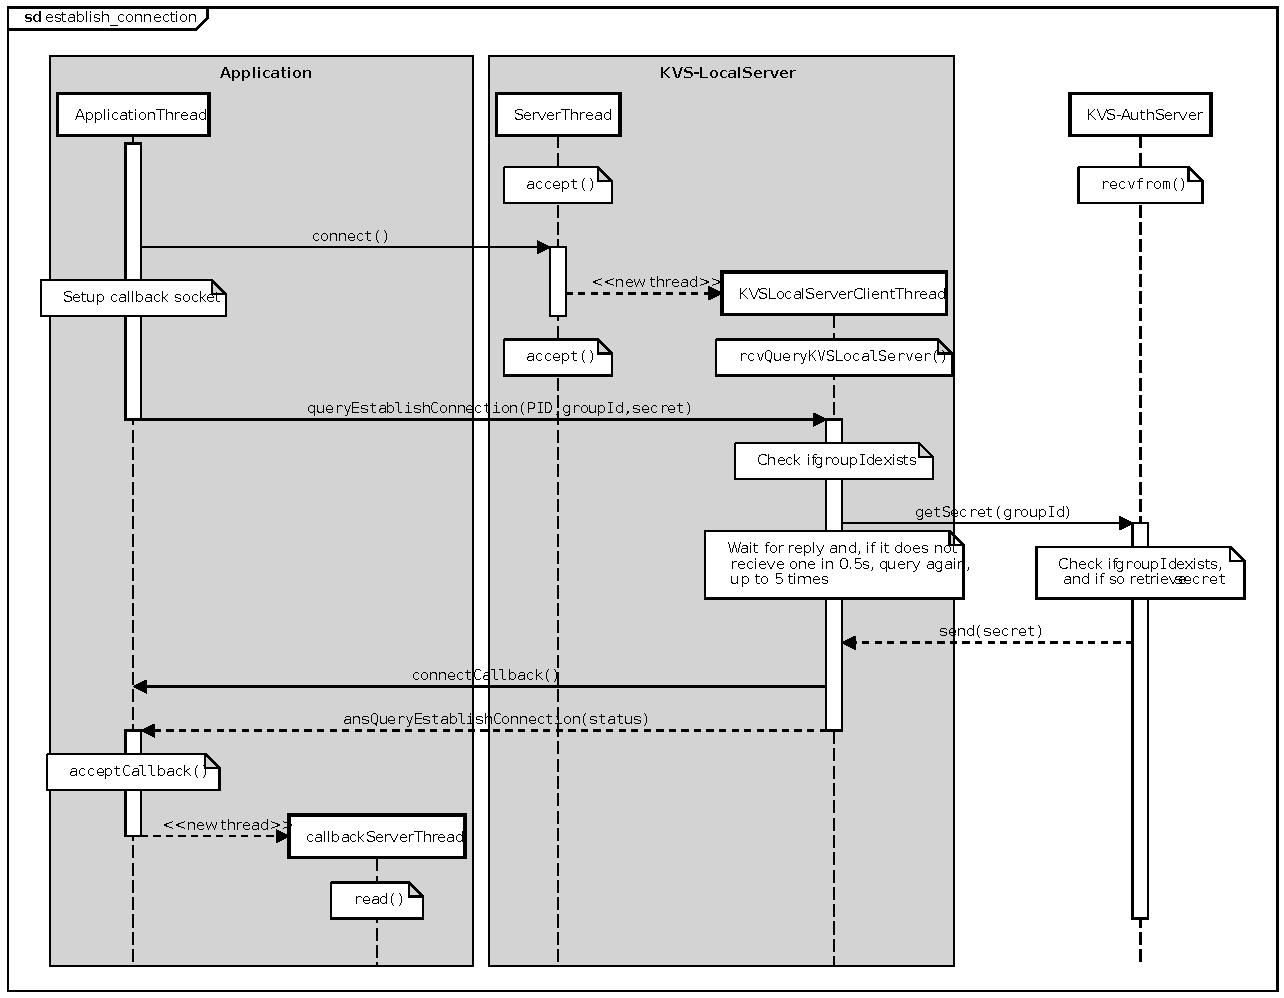
\includegraphics[width=\linewidth]{figures/UML/establish_connection.pdf}
    \caption{Sequence diagram da função \texttt{establish\_connection()} no sistema.}
    \label{fig:sd_establish_connection}
\end{figure}

\begin{figure}[H]
    \centering
    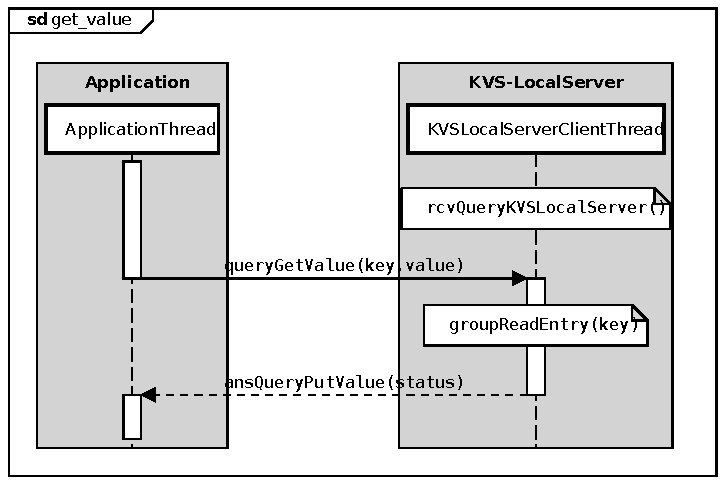
\includegraphics[width=0.7\linewidth]{figures/UML/get_value.pdf}
    \caption{Sequence diagram da função \texttt{get\_value()} no sistema.}
    \label{fig:sd_get_value}
\end{figure}

\begin{figure}[H]
    \centering
    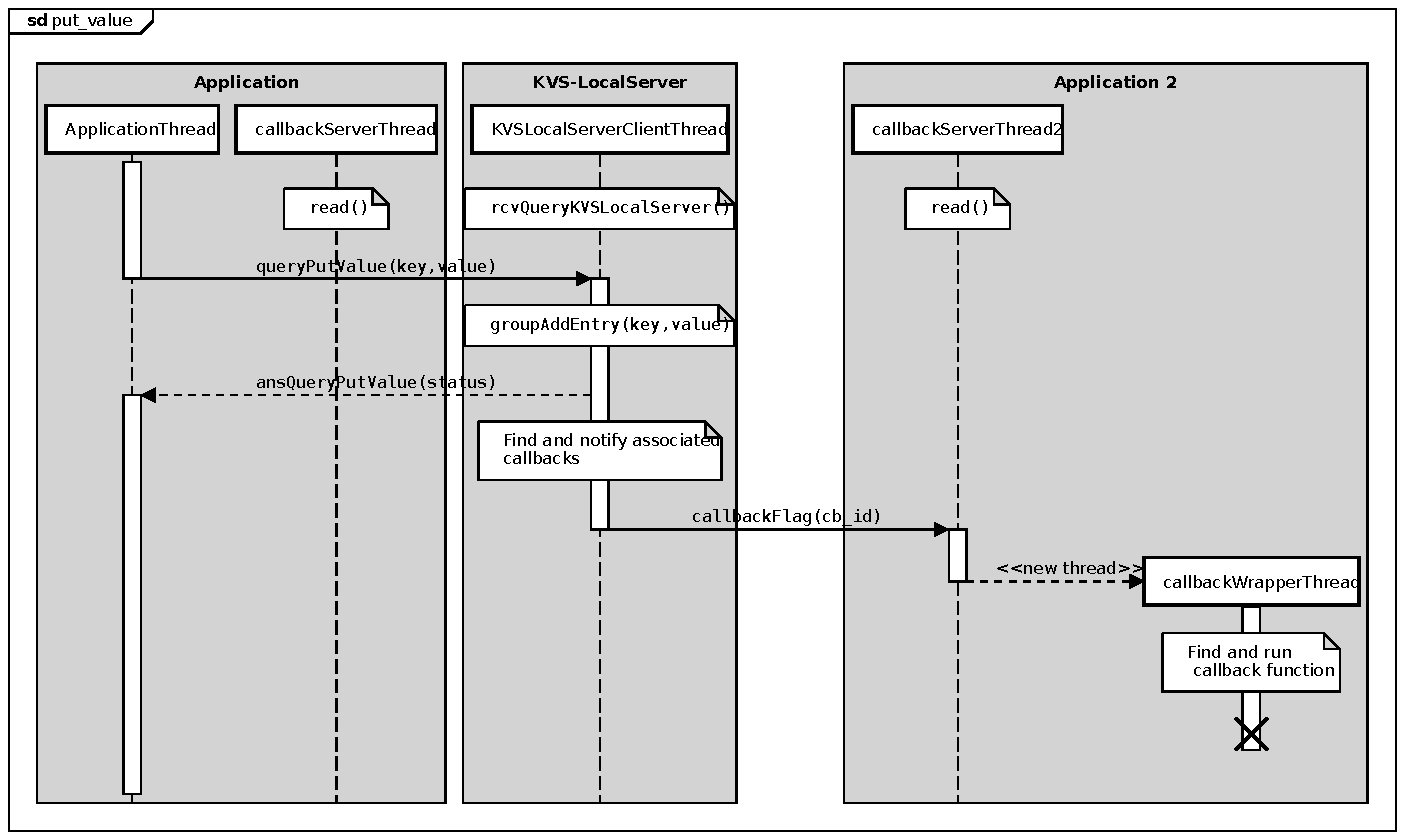
\includegraphics[width=\linewidth]{figures/UML/put_value.pdf}
    \caption{Sequence diagram da função \texttt{put\_value()} no sistema.}
    \label{fig:sd_put_value}
\end{figure}

\begin{figure}[H]
    \centering
    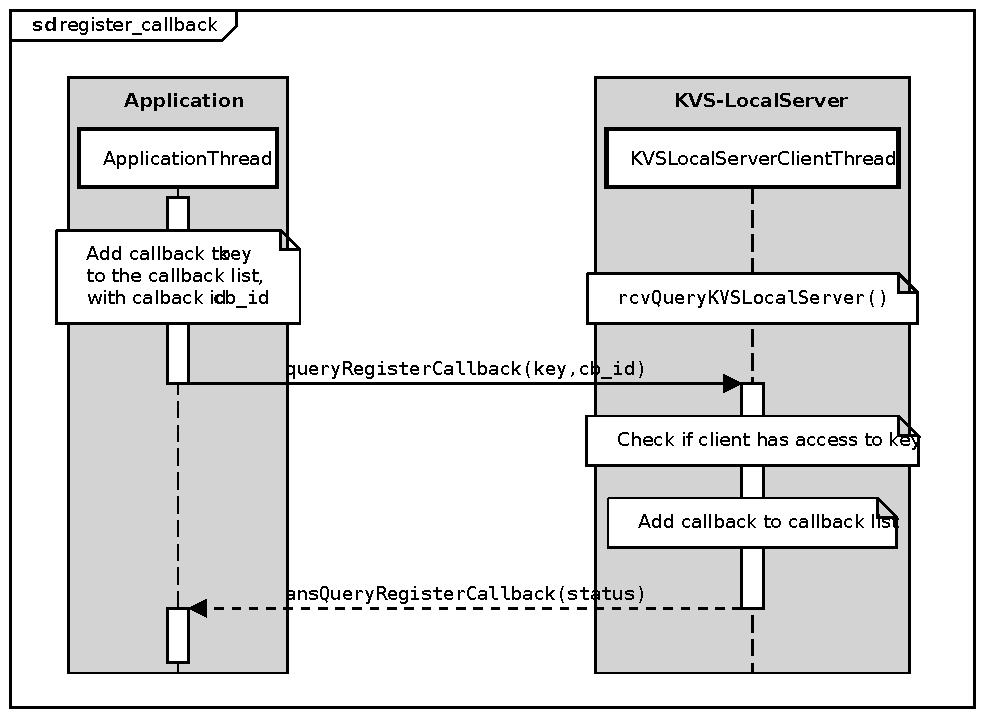
\includegraphics[width=0.8\linewidth]{figures/UML/register_callback.pdf}
    \caption{Sequence diagram da função \texttt{register\_callback()} no sistema.}
    \label{fig:sd_register_callback}
\end{figure}

\begin{figure}[H]
    \centering
    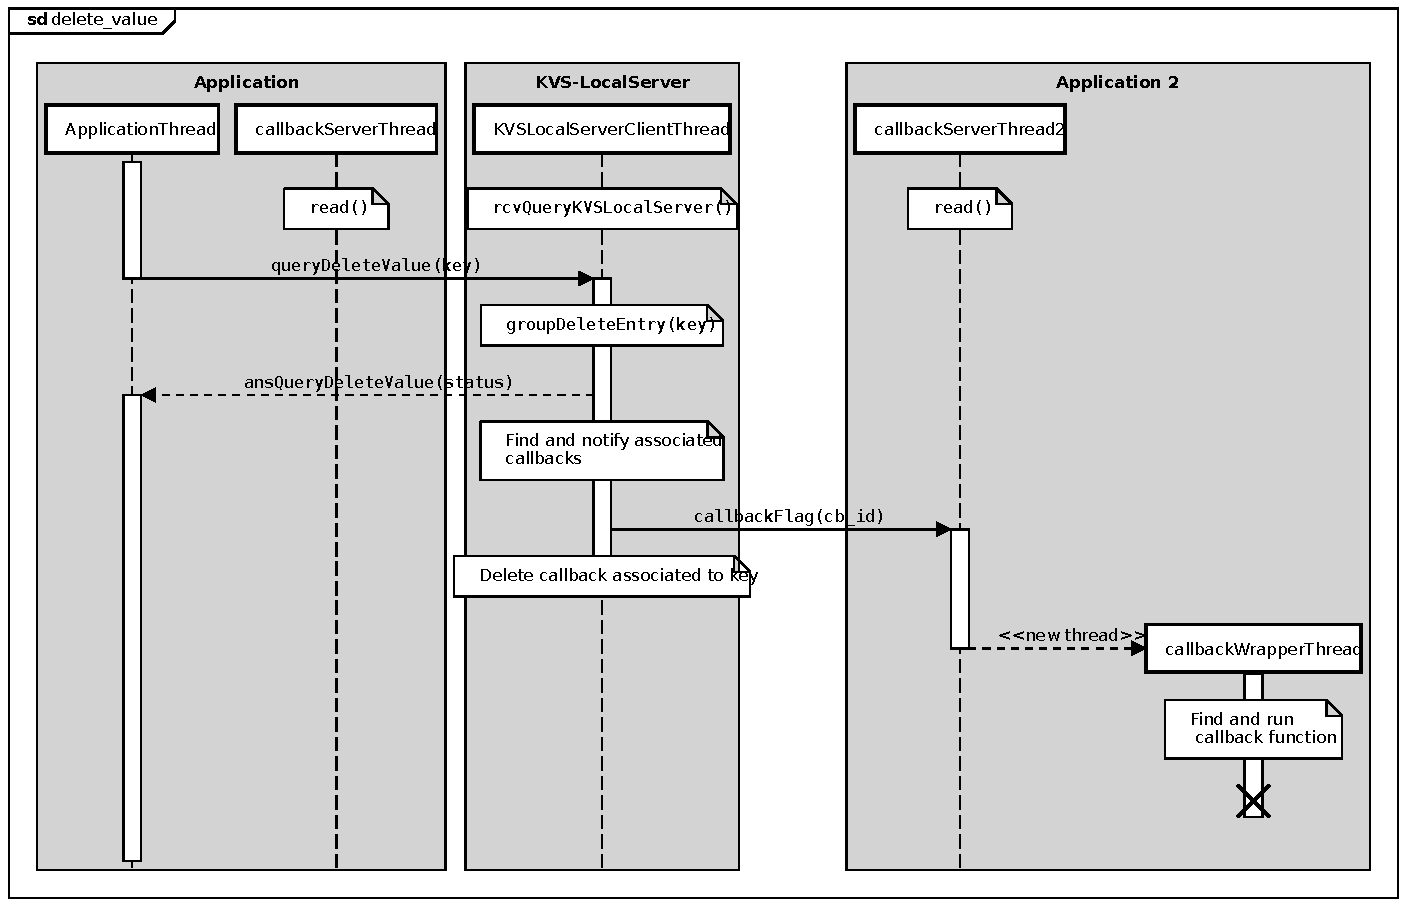
\includegraphics[width=\linewidth]{figures/UML/delete_value.pdf}
    \caption{Sequence diagram da função \texttt{delete\_value()} no sistema.}
    \label{fig:sd_delete_value}
\end{figure}

\begin{figure}[H]
    \centering
    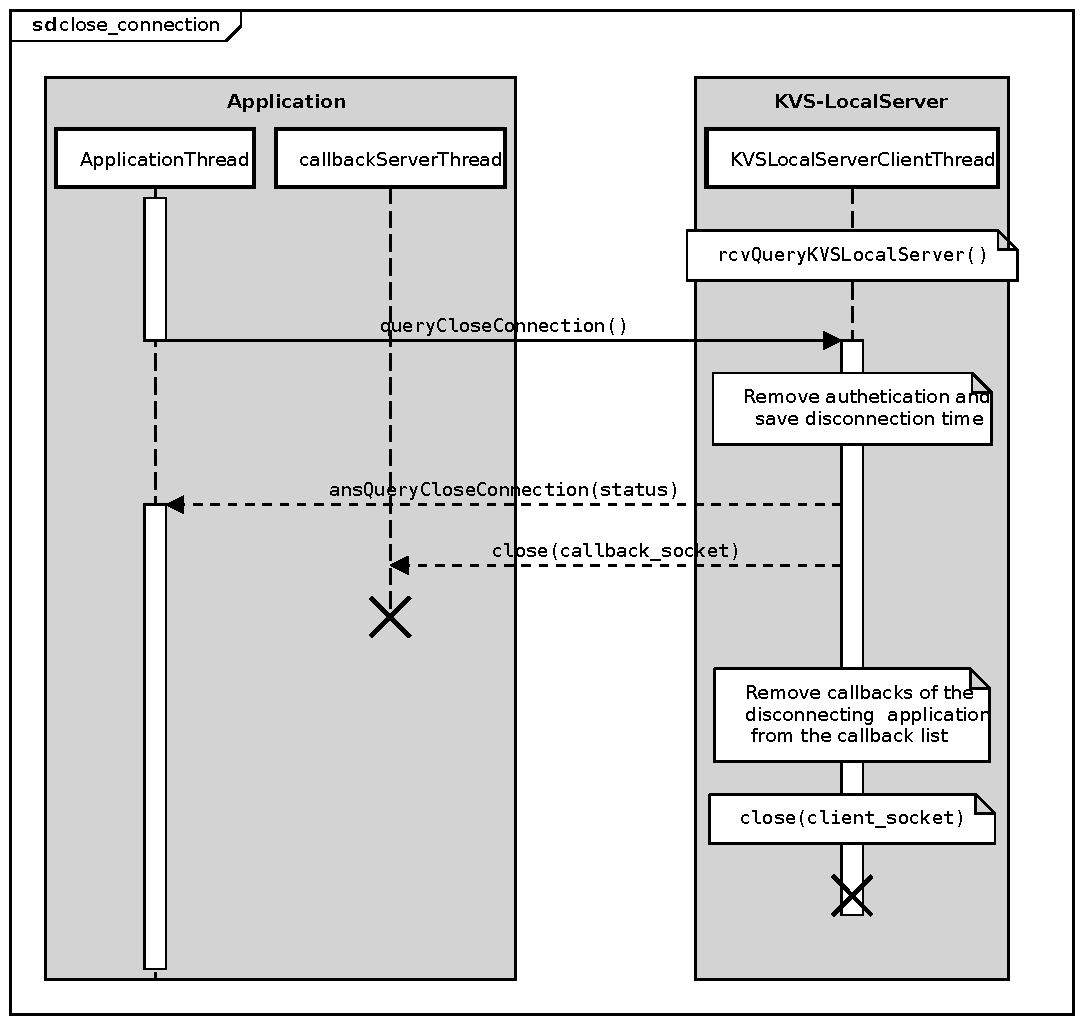
\includegraphics[width=0.7\linewidth]{figures/UML/close_connection.pdf}
    \caption{Sequence diagram da função \texttt{close\_connection()} no sistema.}
    \label{fig:sd_close_connection}
\end{figure}

\section{Comunicação}\label{sec:com}

Nesta secção, documentar-se-ão os diversos protocolos de comunicação entre os subsistemas implementados, apresentando-os de uma forma clara e explicando as razões por detrás das implementações escolhidas.

\subsection{KVS-Lib/KVS-LocalServer}\label{com:lib_local}

% 1. API - KVS LOcal 
% sockets properties (reliability)
% protocolo
% limites

Entre a KVS-Lib e o KVS-LocalServer, a comunicação é realizada através de UNIX domain stream sockets e consideraram-se três possíveis protocolos de comunicação, um dos quais foi o selecionado. No primeiro, as mensagens tinham todas o mesmo tamanho. Este protocolo foi imediatamente excluído porque pretendia-se que o sistema fosse capaz de simultaneamente transmitir chaves com valores muito extensos e chaves com valores muito limitados. Fazê-lo com este protocolo resultaria em grandes perdas de eficiência e em impor limites no tamaho dos values.

No segundo protocolo considerado, as mensagens eram enviadas com um delimitador. No caso particular deste projeto, pretendia-se enviar uma flag (que acabámos por considerar ser uma variável inteira), seguida de possivelmente duas mensagens, como é apresentado na Tabela \ref{tab:args_query_resp}. Como tal, seria necessário colocar o delimitador entre os anteriores campos. Este protocolo, tal como o que foi implementado, estão descritos em \parencite[910-911]{guia_linux}. Tal como aí descrito, observou-se que este protocolo tem como desvantagem o facto de os subsistemas terem de inspecionar os dados que recebem da socket até encontrarem o caractere delimitador. Esta inspeção poder-se-ia fazer byte a byte ou de uma maneira mais eficiente em grupos de bytes de um tamanho selecionado, guardando os bytes que se encontravam depois do último delimitador. De qualquer forma, este método é pouco eficiente.

Como tal, considerou-se o método que em \parencite[910]{guia_linux} é designado por \textit{fixed-size header with a length field}. Este protocolo baseia-se no envio da flag e depois das strings, enviando antes o seu comprimento. Este protocolo tem como vantagem ser bastante mais eficiente em enviar mensagens de tamanho variável como as do sistema em causa neste projeto e como desvantagem o facto de mensagens mal-formadas impedirem a comunicação. Na verdade, a última desvantagem não se aplica ao sistema escolhido pois a comunicação é interior ao sistema. É de notar que mesmo que uma aplicação exterior se conecte ao servidor, não consegue perturbar a comunicação das aplicações que façam uso da KBS-lib, visto que a comunicação através das sockets é privada.
%, pelo que as mensagens apenas poderão ser corrompidas caso existam problemas na execução da KVS-Lib. No caso de serem no KVS-LocalServer, esse seria um problema do administrador. No caso de serem da KVS-Lib, apenas a comunicação com essa KVS-Lib seria afetada pois as restantes são realizadas em diferentes sockets. 
O protocolo de comunicação utilizado é, assim, apresentado na Fig. \ref{fig:KVS-Lib-KVS-LocalServer_com}.

\begin{figure}[ht]
    \centering
    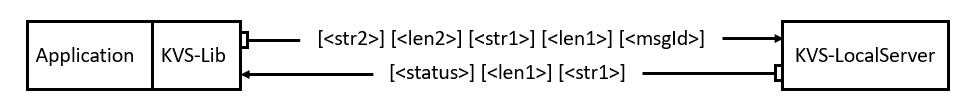
\includegraphics[width=\linewidth]{figures/KVS-Lib-KVS-LocalServer_com_protocol.png}
    \caption{Protocolo de comunicação entre o KVS-Lib e o KVS-LocalServer.}
    \label{fig:KVS-Lib-KVS-LocalServer_com}
\end{figure}

Por último, nota-se o tamanho máximo das mensagens que se podem enviar de acordo com este protocolo. Tendo em conta o protocolo, observa-se que o limite máximo é imposto pelo comprimento enviado. Os tipos das variáveis de comprimento de um pedido são \texttt{int} para o \texttt{<len1>} usado para transmitir uma key e \texttt{uint64\_t} para \texttt{<len2>} usado para trnsmitir um value. O \texttt{<len1>} da resposta é do tipo \texttt{uint64\_t} pois também é utilizado para transmitir um value. Como tal os limites do tamanho das keys e values são impostos por este protocolo de comunicação.  Assim, no que respeita à key o seu tamanho máximo é dado pelo limite máximo de uma variável \texttt{int} (que depende da arquitetura da máquina). Já no que diz repeito ao value, o número máximo de bytes é $2^{64}$ bytes $=2^{34}$ Gbytes, que é bastante acima do que se pode querer, garantindo que qualquer value pode ser enviado. Considerou-se importante definir um valor constante entre arquiteturas para o tamanho do value por se considerar ser um parâmetro que carateriza o sistema.

%C Assim, escolheu-se utilizar uma variável inteira e do tipo \texttt{uint64\_t} para o comprimento,
%omo tal, considera-se importante que este limite seja conhecido e bem definido.

\subsection{Callbacks}\label{com:cb}

Nas Secções \ref{sec:callback_API} e \ref{sec:gestao_cb_local} é detalhada a forma como é feita a implementação dos callbacks do ponto de vista da API e do KVS-LocalServer, repetivamente. Nestas secções é já adiantada o tipo de conexão e a forma e protocolo da comunicação. Por esta razão, nesta secção, é apenas detalhada a forma de estabelecer a conexão dedicada aos callbacks entre a API e o KVS-LocalServer. 

A ligação e criação do canal dedicado para comunicação dos callbacks é feita aquando da chamada de \texttt{establish\_connection} por perte da API. Trata-se de uma ligação de UNIX domain stream sockets. Os passos para o estabelecimento da ligação são os seguintes:
\begin{enumerate}[noitemsep]
    \item Criar a UNIX domain stream socket na API;
    \item Fazer bind da socket a um endeço conhecido tanto pela API como pelo KVS-LocalServer, tendo sido escolhido \texttt{/tmp/cb[PID]};
    \item Fazer \texttt{listen()} para ser possível aceitar ligações;
    \item Enviar o pedido de ligação ao KVS-LocalServer, que inclui o PID, para que seja possível saber o endereço do callback;
    \item Se a autenticação do grupo estiver correta, o KVS-LocalServer cria uma socket e tenta ligar-se à socket do callback;
    \item É enviado o status da operação para a API na resposta ao seu pedido;
    \item Se o status recebido pela API for de sucesso, aceita a ligação do KVS-LocalServer;
    \item É criado na API uma thread dedicada para ler deste canal e detetar um assinalamento de um callback.
\end{enumerate}
Esta sequência de ações pode ser consultada, de forma resumida, no sequence diagram da Fig. \ref{fig:sd_establish_connection}.

% 2. Callbacks
% sockets properties (reliability)
% protocolo
% limites


\subsection{KVS-LocalServer/KVS-AuthServer} \label{sec:com_local_auth}

% 3. KVS Local - Auth
% sockets properties (message oriented)
% How is managed the nondelivery guarantees oft he datagramsockets
% protocolo
% limites

Como apresentado anteriormente, o KVS-LocalServer comunica com o KVS-AuthServer através de INET IPv4 datagram sockets. Estas sockets possibilitam a comunicação através do \textit{TCP/IP protocol suite} que inclui as camadas de \textit{Data-link}, de \textit{Network} baseada em IP, e de \textit{Transport} baseada em UDP. Este mecanismo de comunicação tem as seguintes propriedades:
\begin{enumerate} [noitemsep]
    \item A comunicação é bidirecional;
    \item O endereço de cada \textit{endpoint} é formado por um número de porta e um endereço IPv4;
    \item De acordo com \parencite[1185-1186]{guia_linux}, pode existir fragmentação dos datagrams na camada de IP, o que causa elevadas taxas de perdas de dados e degrada taxas de transferência. De acordo com \parencite[1190]{guia_linux}, programas que queiram efetivamente evitar este problema optam normalmente por usar um limite de 512 bytes para os seus datagrams de UDP. Embora pudessem ser utilizados cerca de 548 bytes evitando na mesma este problema;
    \item De acordo com \parencite[1189]{guia_linux}, UDP adiciona apenas duas funcionalidades ao protocolo IP que são \textit{checksums} para a deteção de erros nos dados transmitidos e números de portas, pelo que herda as restantes caraterísticas do protoclo IP;
    \item De acordo com \parencite[1189]{guia_linux}, o protocolo IP é \textit{unreliable}, \textit{i.e.}, não \say{garante que pacotes são entregues na ordem em que foram transmitidos, que eles não são duplicados, ou mesmo que eles realmente são entregues};
    \item De acordo com \cite{sockets}, uma socket pode-se conectar em 64k portas, de onde as 1-1023 são priveligiadas e as 49152-65535 são dinamicamente associadas a sockets de clientes, pelo que ambos estes intervalos não devem ser utilizados para portas de servidores.
\end{enumerate}
Para além das preocupações de implementação que emanam das anteriores propriedades, é ainda de notar que se deve ter em conta na comunicação entre máquinas diferentes que estas poderão representar dados de formas diferentes. Valores inteiros em diferentes máquinas podem ser representados de formas diferentes de acordo com a ordem dos seus bytes. As duas ordens possíveis são designadas por \textit{big endian} e \textit{little endian}. Para se ter a certeza de que é possível a transmissão de dados entre máquinas com ordens diferentes, foram desenhadas funções de conversão da ordem de cada máquina, \textit{host byte order}, para a ordem da rede, \textit{network byte order}. Estas funções devem ser utilizadas para converter para a ordem da rede antes da transmissão e para converter para a ordem da máquina após a receção.

De qualquer modo, as anteriores propriedades resultam nas seguintes consequências na implementação:
\begin{enumerate}[noitemsep]
    \item A mensagem a enviar entre o KVS-LocalServer e o KVS-AuthServer deverá ter um tamanho inferior, de preferência, a 512 bytes e necessariamente inferior a 548 bytes; \label{item:msg_len}
    \item A necessidade de deteção de erros nos dados não é significativa;
    \item Devem ser implementados mecanismos para evitar a falta de ordem de mensagens; \label{item:msg_disorder}
    \item Devem ser implementados mecanismos para evitar a duplicação de mensagens; \label{item:msg_duplicacao}
    \item Devem ser implementados mecanismos para evitar a falha de entrega de mensagens; \label{item:msg_falha}
    \item As portas a utilizar pelo servidor devem pertencer ao intervalo 1024-49151.
\end{enumerate}

Assim, relativamente ao Ponto \ref{item:msg_len}, começa-se por observar que, tendo em conta que na comunicação o KVS-LocalServer deve pedir ao KVS-AuthServer para tanto apagar um par grupo-segredo como receber o segredo de um par grupo-segredo e que ambas as ações exigem o envio apenas do grupo não seria possível distingui-las pelo que enviam. Desta forma, conclui-se que uma boa solução é enviar, para além do grupo e do segredo na mensagem, também um indicativo da ação a efetuar. Decidiu-se que este indicativo seria uma variável \texttt{int} com os valores das ações definidos no ficheiro de comunicação disponível em ambos os subsistemas, \texttt{KVS\_local-auth\_com.h}. Como tal, a mensagem engloba assim uma variável inteira e duas strings correspondentes ao grupo e ao segredo. Para respeitar o mencionado no Ponto \ref{item:msg_len}, decidiu-se que o comprimento máximo de um segredo e o comprimento máximo de um grupo deveriam ser 256 bytes incluindo o caractere terminador. Para além de permitir cumprir o ponto anterior, este comprimento também não apresenta uma limitação significativa no tamanho de ambas as strings. Em suma, definiu-se a mensagem trocada do KVS-LocalServer para o KVS-AuthServer como na Listing \ref{lst_req_struct}, onde o campo de ID será posteriormente explicado nesta secção.
\begin{lstlisting}[language=C,label={lst_req_struct},caption=Estrutura \texttt{REQ} para a comunicação do KVS-LocalServer para o KVS-AuthServer.]
typedef struct answerStruct{
    // request id
    int id;
    // answer code
    int code;
    // secret
    char secret[MAX_SECRET_LEN];
} ANSWER;
\end{lstlisting}

\subsubsection{Mecanismos de resposta à falta de reliability do UDP} \label{sec:reliability_udp}

Para responder à consequência do Ponto \ref{item:msg_disorder}, decidiu-se simplesmente tratar cada mensagem individualmente no KVS-LocalServer só tratando da mensagem seguinte quando se tinha a certeza de que a mensagem atual já tinha sido completamente processada.

De seguida, para responder aos Pontos \ref{item:msg_duplicacao} e \ref{item:msg_falha}, considerou-se os casos da Fig. \ref{fig:upd_combos}. Comece-se por avaliar o caso da Fig. \ref{fig:udp_combo1}. Neste caso, a mensagem do KVS-LocalServer não é entregue pelo que se poderia criar um grupo no KVS-LocalServer sem o respetivo segredo estar efetivamente guardado no KVS-AuthServer o que levaria a que aplicações não se pudessem ligar a esse grupo. Para evitar este problema, implementaram-se respostas do KVS-AuthServer aos pedidos do KVS-LocalServer. Estas respostas fundem-se com o fornecimento do segredo que antes já era necessário e contêm um código para os diferentes resultados dos pedidos. Por exemplo, um pedido de criação de um novo grupo pode ser respondido com um valor inteiro que corresponde ao erro de o grupo já existir com outro segredo.

Agora que já se percebeu que todos os pedidos devem ser seguidos de uma resposta e não apenas o pedido do segredo de um grupo, passa-se ao caso da Fig. \ref{fig:udp_combo2}. Neste caso, a falha na entrega da mensagem ocorre na resposta ao KVS-LocalServer. Para ultrapassar este problema, implementa-se no KVS-LocalServer a possibilidade de esperar por uma resposta e voltar a enviar um pedido caso ela não seja recebida. Para tal, utiliza-se a opção \texttt{SO\_RCVTIMEO} e a função \texttt{setsockopt} para aplicar um limite de tempo na espera por uma comunicação e um ciclo para impor um determinado número de tentativas. 

No entanto, é de notar que o KVS-AuthServer quando receber a nova tentativa não a distinguirá da anterior e voltará a executá-la, possivelmente com um valor de resposta diferente da anterior. Para resolver este problema, observa-se que para a obtenção de um segredo ou para a eliminação de um grupo tal não será um problema, pois o sistema já deveria estar preparado para entregar vários segredos e receber informação de que um grupo já não existe quando se o queria eliminar é igualmente satisfatório para um sistema que só precisa de assegurar que o grupo foi eliminado. O problema surge na criação de um novo grupo. Na nova tentativa obter-se-ia um erro de \say{grupo já criado}. Isto foi resolvido tendo em conta que na implementação escolhida, o segredo de um novo grupo é criado no KVS-LocalServer e enviado ao KVS-AuthServer, juntamente com o nome do novo grupo. Desta forma, ao verificar se o segredo enviado corresponde ao do grupo já criado a nossa confiança de que o que se verificou foi realmente uma falha de entrega da resposta aumenta. Esta foi a razão pela qual se escolheu criar o segredo no KVS-LocalServer.

O caso da Fig. \ref{fig:udp_combo3} corresponde à duplicação de mensagens no KVS-LocalServer sem entrega de respostas do KVS-AuthServer. Este problema leva a que a mesma ação seja repetida no KVS-AuthServer, o que já se viu não resultar num problema. Como tal, este caso é semelhante ao da Fig. \ref{fig:udp_combo2}.

O caso da Fig. \ref{fig:udp_combo4} corresponde à duplicação de mensagens no KVS-LocalServer e entrega de apenas uma das respostas. Este caso pode dividir-se em dois. Num primeiro, a resposta perdida é a do primeiro pedido a ser processado, pelo que o caso equivale ao caso em que uma mensagem é enviada, a resposta é perdida, e uma nova mensagem é enviada outra vez. Este caso já foi resolvido. No segundo, a resposta perdida é a do segundo pedido a ser processado, pelo que se recai num caso de transmissão normal.

O caso da Fig. \ref{fig:udp_combo5} corresponde à duplicação de mensagens no KVS-LocalServer com resposta a ambas as mensagens. Neste caso, a primeira resposta a ser processada é bem processada mas a segunda resposta é deixada por ser recebida no KVS-LocalServer, pelo que na próxima receção a segunda resposta será lida. Para evitar que ela seja interpretada como a resposta a um pedido seguinte é implementado o ID de pedido já mostrado na Listing \ref{lst_req_struct}. Assim, um KVS-LocalServer apenas aceita como resposta a um pedido uma resposta que contenha o mesmo ID que o pedido.

O caso da Fig. \ref{fig:udp_combo6} corresponde à duplicação de respostas no KVS-AuthServer sem que elas cheguem ao KVS-LocalServer. Este caso recai no caso da Fig. \ref{fig:udp_combo2}. Por sua vez, o caso da Fig. \ref{fig:udp_combo7} recai no caso de uma transmissão normal e o da Fig. \ref{fig:udp_combo8} recai no caso da Fig. \ref{fig:udp_combo5}.

\begin{figure}[ht]
    \centering
    \begin{subfigure}[b]{0.49\textwidth}
         \centering
         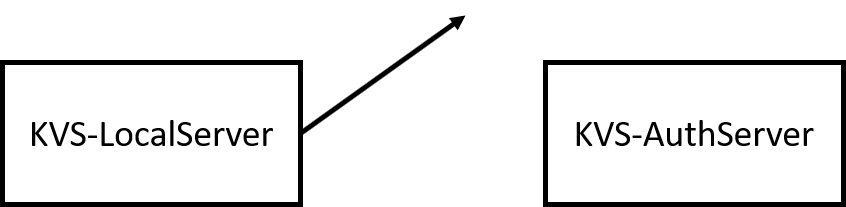
\includegraphics[width=\textwidth]{figures/udp_combo1.png}
         \caption{KVS-LocalServer envia mas não é entregue.}
         \label{fig:udp_combo1}
    \end{subfigure}
    \hfill
    \begin{subfigure}[b]{0.49\textwidth}
         \centering
         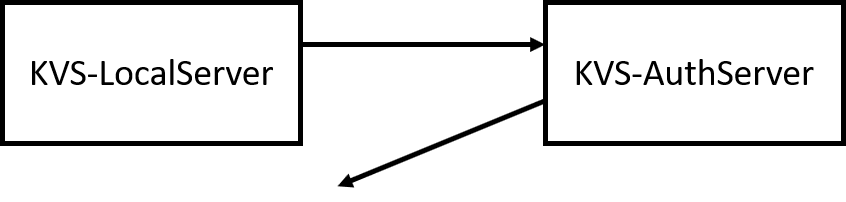
\includegraphics[width=\textwidth]{figures/udp_combo2.png}
         \caption{A resposta do KVS-AuthServer não é entregue.}
         \label{fig:udp_combo2}
    \end{subfigure}
    \\ \vspace{0.2cm}
    \begin{subfigure}[b]{0.49\textwidth}
         \centering
         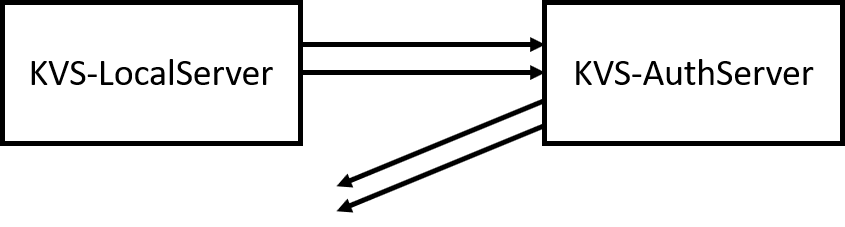
\includegraphics[width=\textwidth]{figures/udp_combo3.png}
         \caption{O pedido do KVS-LocalServer é duplicado e as respostas do KVS-AuthServer não são ambas entregues.}
         \label{fig:udp_combo3}
    \end{subfigure}
    \hfill
    \begin{subfigure}[b]{0.49\textwidth}
         \centering
         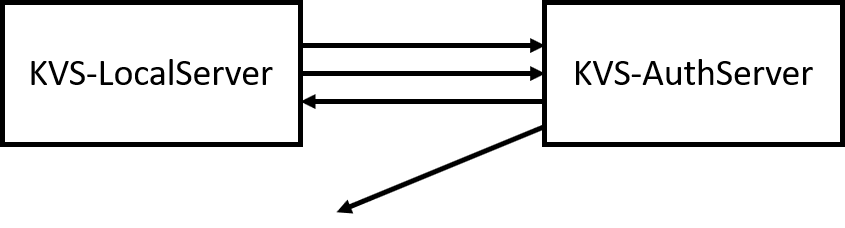
\includegraphics[width=\textwidth]{figures/udp_combo4.png}
         \caption{O pedido do KVS-LocalServer é duplicado e apenas uma das respostas do KVS-AuthServer é entregue.}
         \label{fig:udp_combo4}
    \end{subfigure}
    \\
    \begin{subfigure}[b]{0.49\textwidth}
         \centering
         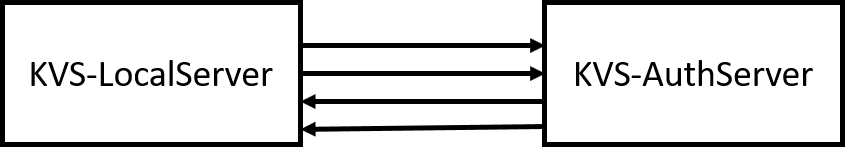
\includegraphics[width=\textwidth]{figures/udp_combo5.png}
         \caption{O pedido do KVS-LocalServer é duplicado e ambas as respostas do KVS-AuthServer são entregues.}
         \label{fig:udp_combo5}
    \end{subfigure}
    \hfill
    \begin{subfigure}[b]{0.49\textwidth}
         \centering
         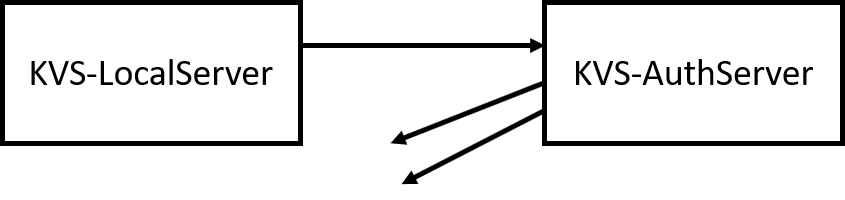
\includegraphics[width=\textwidth]{figures/udp_combo6.png}
         \caption{A resposta do KVS-AuthServer é duplicada e nenhuma é entregue.}
         \label{fig:udp_combo6}
    \end{subfigure}
    \\
    \begin{subfigure}[b]{0.49\textwidth}
         \centering
         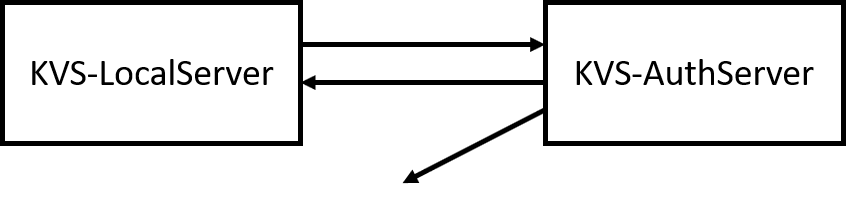
\includegraphics[width=\textwidth]{figures/udp_combo7.png}
         \caption{A resposta do KVS-AuthServer é duplicada e apenas uma é entregue.}
         \label{fig:udp_combo7}
    \end{subfigure}
    \hfill
    \begin{subfigure}[b]{0.49\textwidth}
         \centering
         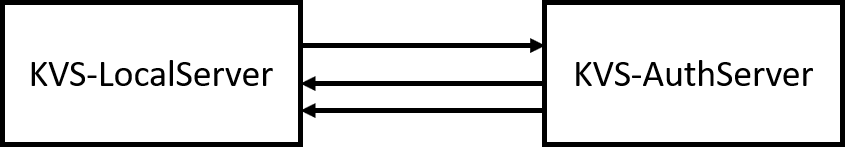
\includegraphics[width=\textwidth]{figures/udp_combo8.png}
         \caption{A resposta do KVS-AuthServer é duplicada e ambas são entregues.}
         \label{fig:udp_combo8}
    \end{subfigure}
    \caption{Combinações de erros devidas à falta de \textit{reliability} do UDP.}
    \label{fig:upd_combos}
\end{figure}

Para terminar o presente tópico, apresenta-se apenas a estrutura de dados da resposta do KVS-AuthServer ao KVS-LocalServer na Listing \ref{lst_ans_struct}.
\begin{lstlisting}[language=C,label={lst_ans_struct},caption=Estrutura \texttt{ANS} para a comunicação do KVS-AuthServer para o KVS-LocalServer.]
typedef struct answerStruct{
    // request id
    int id;
    // answer code
    int code;
    // secret
    char secret[MAX_SECRET_LEN];
} ANSWER;
\end{lstlisting}

\subsubsection{Algumas preocupações de segurança}

Outro conjunto de preocupações a ter em conta são preocupações de segurança. Embora no KVS-AuthServer já se tenha falado da receção de mensagens de entidades externas ao sistema, nesse subsistema elas poderiam ser apenas ignoradas sem grande aumento de complexidade. No KVS-LocalServer, tal já não acontece. Devido ao protocolo de pedidos e respostas implementado, quando o KVS-LocalServer espera por respostas, ele pode receber respostas de outra entidade que conheça o seu IP e porta. Assim, caso não se verifique o remetente de cada resposta, incorre-se na possibilidade de perder respostas do próprio KVS-AuthServer, já que se receberiam as do remetente anónimo e passar-se-ia para um pedido noutra thread ou o pedido seguinte na mesma thread. Desta forma, decidiu-se verificar quem é o remetente de cada mensagem enviada (para além de se o ID do pedido corresponde ao da mensagem) num ciclo antes de sair da zona crítica de envio e receção.

\section{Paralelismo} \label{sec:synch}

Como detalhado nas secções anteriores, os subsistemas são implementados com recurso a várias threads que partilham memória entre si. Assim, nesta a secção serão apresentados os métodos de sincronização para permitir integridade nos dados e proteger os acessos a variáveis partilhadas. Ainda que já tenha sido mencionado anteriormente como é que a divisão em várias threads é implementada para cada subsistema, esta será resumida brevemente.

\subsection{KVS-Lib}
Na KVS-Lib API a gestão de threads é implemementada, resumidadmente, utilizando
\begin{enumerate}[noitemsep]
    \item Uma thread dedicada para ler da socket de callbacks;
    \item Uma thread dedicada para procurar e executar cada callback que seja assinalado.
\end{enumerate}
Para além disso, KVS-Lib API é implementada para ser thread-safe, nesse sentido têm de ser implementados mecanismos de sincronização que permitam que as funções da API possam ser invocadas por várias threads em simultâneo.

\subsubsection{Comunicação}
Em primeiro lugar, como referido anteriormente, as invocações das funções da API sevem ser thread-safe. Nesse sentido, como as UNIX domain stream sockets não são orientadas para a receção e envio de mensagens, é necessário garantir que chamadas de funções da API em simultâneo em threads distintas usam o canal de comunicação sem perturbar o protocolo de outras chamadas ou consumir as respostas direccionada a elas.

Nesse sentido, por uma questão de simplicidade, optou-se por implementar uma região crítica para cada pedido e leitura da resposta correspondente. Dito de outras palavras, antes de ser feito um pedido ao KVS-LocalServer, é bloqueada a região crítica que só é libertada após ter sido recebida a resposta do servidor. O seu uso é exemplificado na Listing \ref{lst_mtx_com_lib}.
\begin{lstlisting}[language=C,label={lst_mtx_com_lib},caption= Uso de uma região crítica para a integridade de comunicação entre KVS-Lib e KVS-LocalServer (\texttt{KVS-lib-com.c}).]
    //(...)
     pthread_mutex_lock(&com_mtx);
    // Protocol for communication with server:
    // 1. Write message identification
    //(...)
    // 2. Write size of first string
    //(..)
    // 3. Write first string
    //(...)
    // 4. Write size of second string
    //(...)
    // 5. Write second string
    //(...)
    // 6. Read status message
    //(...)
    // 7. If response contains string response read it
    //(...)
    pthread_mutex_unlock(&com_mtx);
    //(...)
\end{lstlisting}

\subsubsection{Lista de callbacks}
Outro conjunto de dados que requer sincronização no seu acesso é a lista de callbacks. Esta é acedida:
\begin{enumerate}[noitemsep]
    \item Através da função \texttt{callbackAdd} em \texttt{KVS-lib-cb.c} - por qualquer thread da aplicação que registe um callback, usando \texttt{register\_callback()}, adicionando um bloco à lista;
    \item Através das threads \texttt{callbackWrapperThread} em \texttt{KVS-lib-cb.c} - que são criadas quando é assinalado um callback, que leêm apenas a lista;
    \item Através da função \texttt{callbackClear} em \texttt{KVS-lib-cb.c} - pela thread que lê os assinalamentos dos callbacks, quando é fechada a ligação com \texttt{close\_connection()} ou é detetado um erro no canal dedicado aos callbacks.
\end{enumerate}
Assim, visto que não há perda de integridade dos dados se a lista for lida simultaneamente, que é o que acontece se forem assinalados dois callbacks em simultâneo, serão usados read/write locks, ao invés de uma região exclusiva. Assim, 
\begin{enumerate}[noitemsep]
    \item Como podem ser feitas adições simultâneas, em \texttt{callbackAdd} tem de ser usado um write lock ao adicionar um bloco à lista;
    \item Visto que não há perda de integridade dos dados se a lista for lida simultaneamente, em \phantom{jbjkbjbj} \texttt{callbackWrapperThread} é usado um read lock ao procurar o callback na lista;
    \item Ao eliminar a lista, como ainda há forma de outras threads estarem a tentar aceder a ela, em \texttt{callbackClear} tem de ser usado um write lock.
\end{enumerate}

Note-se ainda que a região bloqueada é mantida a um mínimo. Dentro das regiões críticas são apenas feitas alterações à estrutura da lista. Alocações de novos blocos e libertação de memória, por exemplo, são efetuados fora dela.

\subsection{KVS-LocalServer}
No KVS-LocalServer a gestão de threads é implementada, resumidadamente, utilizando
\begin{enumerate}[noitemsep]
    \item Uma thread para ler e executar os pedidos que o administrador faz na consola;
    \item Uma thread para aceitar connections de clientes;
    \item Uma thread para cada aplicação, que lê, processa, e responde a pedidos dessa aplicação;
    \item Uma thread para implementar o shutdown controlado.
\end{enumerate}
Estas threads partilham memória entre si, nomeadamente: i) a lista de grupos; ii) as listas de key-value pairs; iii) a lista de clientes; iv) o apontador do grupo a que cada cliente está autenticado; e v) a lista de callbacks. Desta forma, todos os acessos a estes dados partilhados devem ser sincronizados de forma a preservar a integridade dos dados.

\subsubsection{Lista de grupos}
Em primeiro lugar trata-se a sincronização de acessos à lista de grupos. Esta é acedida:
\begin{enumerate}[noitemsep]
\item Através da função \texttt{groupAdd} em \texttt{KVSLocalServer-data.c} - por uma única thread que executa os comandos da UI;
\item Através da função \texttt{groupDelete} em \texttt{KVSLocalServer-data.c} - por uma única thread que executa os comandos da UI;
\item Através da função \texttt{groupShow} em \texttt{KVSLocalServer-data.c} - por uma única thread que executa os comandos da UI;
\item Através da função \texttt{groupCheckExistence} em \texttt{KVSLocalServer-data.c} - por várias threads das aplicações;
\item Através da função \texttt{groupClear} em \texttt{KVSLocalServer-data.c} - pela thread dedicada ao shutdown.
\end{enumerate}

É de notar que há também acessos a blocos da lista diretamente a partir de apontadores guardados na estrutura de cada cliente. Estes acessos são, no entanto, geridos de outra forma, como detalhado nas duas próximas subsecções.

Assim, visto que não há perda de integridade dos dados se a lista for lida simultaneamente será usada uma variável global de sincronização read/write lock dedicada para a lista de grupos, ao invés de uma região exclusiva. Assim, 
\begin{enumerate}[noitemsep]
    \item Como não podem ser feitas adições simultâneas, dado que só uma thread pode adicionar grupos, em \texttt{KVSLocalServer-data.c} pode apenas ser usado um read lock ao adicionar um bloco à lista;
    \item Para eliminar um grupo as ligações da lista terão de ser alteradas, logo em  \texttt{groupDelete} tem de ser usado em write lock;
    \item Para percorrer a lista e ler informação de um grupo, em \texttt{groupCheckExistence}  é usado apenas um read lock;
   \item Para eliminar todos os grupos em  \texttt{groupClear} é usado um write-lock.
\end{enumerate}

Note-se ainda que a região bloqueada é mantida a um mínimo. Dentro das regiões críticas são apenas feitas alterações à estrutura da lista. Alocações de novos blocos e libertação de memória, por exemplo, são efetuadas fora dela. Aliás, na criação de um grupo, a alocação do bloco é feita antes de entrar na região cítica, mesmo que haja a possibilidade de não ser necessário alocar memória, se o grupo já existir. Assim, consegue-se libertar as regiões críticas mais rapidamente.

\subsubsection{Acesso autenticado de clientes a um grupo}\label{sec:authgroup}
Em segundo lugar, trata-se da sincronização do acesso de cada cliente à memória do grupo em que está autenticado. Como é dito na Secção \ref{sec:gestao_clientes} cada cliente tem acesso ao apontador para o bloco do grupo ao qual está autenticado. Note-se que esta configuração tem vantagens significativas como: i) de cada vez que tem de ser feito o acesso por parte de um cliente a um key-value pair não é necessário percorrer toda a lista de grupos à procura do grupo autenticado; ii) não é necessário aceder à região crítica da lista de grupos, permitindo, portanto uma aplicação aceder a informação do seu grupo enquanto um grupo distinto está a ser eliminado ou está um grupo a ser criado. Este aumento de performance vem, naturalmente, com um aumento na complexidade dos mecanismos de sincronização. 

Assim, na estrutura de cada cliente, detalhada na Secção \ref{sec:gestao_clientes} é incluída uma variável de sincronização de acessos de cada cliente ao seu grupo autenticado, para proteger os seus acessos à memória. Este tem como principal objetivo garantir a validade do apontador para o bloco de grupo, se o grupo foi eliminado e for feito um acesso simultâneo. Nesta secção o procedimento de apagar um grupo é explicado com mais detalhe.

Para além disso, só duas threads podem aceder à variável de acesso de um cliente ao seu grupo autenticado: i) a thread que executa as ações da UI; e ii) a thread que recebe, processa, e responde a pedidos desse cliente. Assim, não é vantajoso um read write lock, usa-se portanto um mutex.

É necessário proteger o acesso de um cliente ao seu grupo autenticado nas seguintes circunstâncias:
\begin{enumerate}[noitemsep]
    \item Em todos os acessos que a thread de um cliente faz ao seu grupo autenticado (ler, ou escrever key-value pair por exemplo), \textit{i.e.}, sempre que fizer uso do apontador \texttt{authGroup};
    \item Quando um grupo é eliminado.
\end{enumerate}

Note-se que antes de cada acesso e depois de entrar na região crítica é necessário verificar a validade do endereço, visto que este pode estar a \texttt{NULL} caso não haja um acesso autorizado ou o grupo tenha sido apagado.

Usando esta configuração é possível apagar um grupo e manter a integridade de toda a memória partilhada e dos acessos a dados. Assim, o procedimento de apagar um grupo segue os seguintes passos (função \texttt{groupDelete} em \texttt{KVSLocalServer-data.c}):
\begin{enumerate}[noitemsep]
    \item Notificar o KVS-AuthServer para eliminar o grupo na sua memória;
    \item Procurar o grupo e religar a lista de forma a que o bloco não possa ser acedido (com write lock na varável de proteção da lista de grupos);
    \item Retirar o acesso de todos os clientes autenticados a este grupo, pondo a variável \texttt{authGroup} a \texttt{NULL} (com o bloqueio das região crítica que protege esta variável de acesso, como indicado acima);
    \item Destruir a região crítica de acesso às key-value pairs dessse grupo, visto que já nada consegue aceder a ela;
    \item Libertar a memória da lista de key-value pairs;
    \item Libertar a memória do bloco do grupo.
\end{enumerate}

\subsubsection{Lista de key-value pairs}
Em segundo lugar trata-se a sincronização de acessos à lista de key-value pairs. Esta é acedida em \texttt{KVSLocalServer-data.c}:
\begin{enumerate}[noitemsep]
\item Através da função \texttt{groupAddEntry} - por várias threads das aplicações;
\item Através da função \texttt{groupReadEntry} - por várias threads das aplicações;
\item Através da função \texttt{groupDeleteEntry} - por várias threads das aplicações;
\item Através da função \texttt{entriesDelete} - por várias threads das aplicações.
\end{enumerate}

Assim, visto que não há perda de integridade dos dados se a lista for lida simultaneamente será usada uma variável de sincronização read/write lock dedicada para cada lista de key-value pairs, ao invés de uma região exclusiva. Esta variável é guardada na estrutura de grupo, como detalhado na Secção \ref{sec:gestao_dados}. Assim:
\begin{enumerate}[noitemsep]
    \item Como podem ser feitas adições simultâneas, em \texttt{groupAddEntry} tem de ser usado write lock ao adicionar um bloco à lista;
    \item Em \texttt{groupReadEntry} é usado um read lock;
    \item Em \texttt{groupAddEntry} tem de ser usado write lock ao adicionar um bloco à lista;
   \item Para eliminar todos os grupos em  \texttt{groupClear} é usado um write-lock.
\end{enumerate}

Mais uma vez, a região bloqueada é mantida a um mínimo. Dentro das regiões críticas são apenas feitas alterações à estrutura da lista. Alocações de novos blocos e libertação de memória, por exemplo, são efetuados fora dela. Aliás na criação de um key-value pair, a alocação do bloco é feita antes de entrar na região crítica, mesmo que haja a possibilidade de não ser necessário alocar memória, se o key-value pair já existir. Assim, consegue-se libertar as regiões críticas mais rapidamente.

\subsubsection{Lista de clientes}
Por fim, é também necessário proteger o acesso à lista de clientes e à memória do bloco de cada cliente. Há acessos à:
\begin{enumerate}[noitemsep]
    \item Memória do bloco de cada grupo executados unicamente por uma thread, a thread que recebe, processa, e responde aos pedidos desse cliente;
    \item Lista através da função \texttt{clientAdd} em \texttt{KVSLocalServer-client.c} - por uma única thread que está dedicada a aceitar a conexões de novas aplicações;
    \item Lista através da função \texttt{clientShow} em \texttt{KVSLocalServer-client.c} - por uma única thread que está dedicada a ler e processar comandos do administrador do KVS-LocalServer;
    \item Lista através da função \texttt{closeClients} em \texttt{KVSLocalServer-client.c} - por uma única thread que está dedicada ao shutdown controlado do KVS-LocalServer;
    \item Lista através da função \texttt{clientDeleteAccessGroup} em \texttt{KVSLocalServer-client.c} quando é eliminado em grupo, por uma única thread que está dedicada a ler e processar comandos do administrador do KVS-LocalServer;
\end{enumerate}

Foi utilizada uma aquitetura de forma a que acessos à lista possam ser sincronizados de forma distinta dos acessos à memória. Por um lado, pretende-se, por uma questão de eficiência, que não se tenha que usar regiões críticas no acesso a dados dentro da estrutura de cada cliente, onde está armazenado o file descriptor da socket, por exemplo. (Uma execeção a esta guideline é a variável \texttt{authGroup} que como está descrito na Secção \ref{sec:authgroup} tem de ser protegida com uma região crítica dedicada). Assim para tal: i) só uma thread pode aceder ao conteúdo de um bloco da lista de cliente; e ii) sempre que elimina um bloco de um cliente, primeiro é feito \texttt{pthread\_join} da thread que tem acesso à memória do bloco e só depois se apaga o bloco da lista. Assim, é possível garantir a integridade do conteúdo de cada bloco de forma eficiente usando \texttt{pthread\_join} em vez de uma região crítica para sincronização. 

Por outro lado, para a sincronização das ligações da lista, nota-se que a adição de um novo cliente e a leitura da lista pode ser feita em simultâneo, pelo que poderá ser usado um read/write lock (da mesma forma que foi usado nas listas acima). No entanto, como apenas o comando de mostrar um grupo na consola do KVS-LocalServer (que é corrido muito poucas vezes) pode correr em simultâneo com a adição de grupo, o uso de um read/write lock em vez de um mutex não traz um aumento de performance significativo. Por uma questão de simplicidade, foi usado um mutex para proteger os acessos à lista descritos acima. Note-se, novamente, que as regiões críticas são o mais curtas possível de forma a bloquear o acesso de outras threads o menor tempo possível.

\subsubsection{Lista de callbacks}
Por fim, é também necessário proteger o acesso à lista de callbacks. Esta é acedida:
\begin{enumerate}[noitemsep]
    \item Através da função \texttt{callbackRegister} em \texttt{KVSLocalServer-cb.c} - pelas threads dos clientes quando estes chamam \texttt{register\_callback()}, adicionando um bloco à lista;
    \item Através da função \texttt{callbackDeleteKey} em \texttt{KVSLocalServer-cb.c} - pelas threads dos clientes quando uma key é apagada;
    \item Através da função \texttt{callbackDeleteClient} em \texttt{KVSLocalServer-cb.c} - pelas threads dos clientes quando a ligação é fechada de forma comandada ou descomandada, por forma a apagar todos os callbacks associados o cliente recém desconectado;
    \item Através da função \texttt{callbackFlag} em \texttt{KVSLocalServer-cb.c} - pelas threads dos clientes quando é pedida a alteração de uma key, de forma a notificar os callbacks associados.
\end{enumerate}
Mais uma vez, à semelhança da lista de grupos e de key-value pairs, visto que não há perda de integridade dos dados se a lista for lida simultaneamente, que é o que acontece se forem assinalados dois callbacks em simultâneo, serão usados read/write locks, ao invés de uma região exclusiva. Assim, 
\begin{enumerate}[noitemsep]
    \item Como podem ser feitas adições simultâneas, em \texttt{callbackRegister} tem de ser usado um write lock ao adicionar um bloco à lista;
    \item Ao eliminar a lista, como ainda há forma de outras threads estarem a tentar aceder a ela, em \texttt{callbackDeleteKey} e \texttt{callbackDeleteClient} têm de ser usados write locks ao eliminar o bloco da lista.
    \item Visto que não há perda de integridade dos dados se a lista for lida simultaneamente, em \phantom{jbjkbjbj} \texttt{callbackFlag} é usado um read lock ao adicionar um bloco à lista;
\end{enumerate}

Mais uma vez, à semelhança do que foi descrito para a sincronização da listas acima, as mesmas técnicas foram usadas para manter as regiões críticas a um mínimo.

\subsubsection{Comunicação com o KVS-AuthServer}

Na comunicação com o KVS-AuthServer também é necessário implementar mecanismos de sincronização, pois, tal como se observou na Secção \ref{sec:com_local_auth}, o KVS-LocalServer deve i) receber uma resposta e ii) enviar um número de pedido juntamente com um pedido. Para solucionar i), é necessário que cada thread do KVS-LocalServer envie um pedido e espere pela resposta sem interrupções. Como tal, observou-se que era necessário implementar uma região crítica em torno do envio do pedido e até se terminar a receção da resposta (a receção da resposta pode ser terminada por um erro, por se ter expirado a duração da espera, ou por se ter recebido a resposta). Para solucionar ii), decidiu-se que a forma que permite ter números de pedido consistentemente diferentes entre pedidos é a de continuamente incrementar uma variável inteira. Como tal, é necessário implementar um mecanismo de sincronização para que cada thread possa seguramente receber e incrementar o número de pedidos. Ambas as regiões críticas anteriores foram implementadas com recurso a mutexes.

\subsection{KVS-AuthServer}

Como já explicado anteriormente, o KVS-AuthServer apresenta apenas uma thread, sendo esta a forma de resolver preocupações de sincronização. Assim, permite-se que o KVS-AuthServer esteja sempre a tratar de um único pedido desde a sua receção até à resposta. No entanto, na verdade, se se quisesse aumentar a capacidade de resposta do KVS-AuthServer poder-se-ia simplesmente criar mais threads que executassem o ciclo principal da main tendo todas acesso aos dados. Tal exigiria a implementação de mecanismos de sincronização no acesso aos dados, o que não seria problemático, uma vez que já foi implementado um mecanismo semelhante no KVS-LocalServer. Assim, considera-se que esta solução poderia ter sido implementada para mostrar que a capacidade de resposta pode ser escalada.

\section{Validação}

%% Valgrind e memoria
% Ficheiros grandes
% falar dos exemplos e bashes

Para realizar os testes e a validação do sistema desenvolvido, escreveram-se também vários ficheiros de exemplos e scripts para os compilar e executar. Os scripts desenvolvidos consistiam em:
\begin{enumerate} [noitemsep]
\item Um único cliente que executa as funções da KVS-Lib, compilado e executado no script \\ \texttt{runSimpleClient.sh};
\item Um ficheiro que cria vários processos filho e testa as funções da KVS-Lib, compilado e executado no script \texttt{runMultiClients.sh};
\item Um ficheiro que criava várias threads e testava a sincronização do sistema compilado e executado no script \texttt{runThreadMadness.sh};
\item Dois ficheiros que testam o funcionamento dos callbacks, compilado e executado nos scripts \texttt{runCallbackTest.sh} e \texttt{runCallbackTest\_createkey.sh};
\item Um ficheiro que testa o envio de grandes ficheiros de texto, compilado e executado no script \texttt{runFileTransfer.sh}.
\end{enumerate}

Nos ficheiros anteriores, é apenas de notar que os ficheiros \texttt{runCallbackTest\_createkey.sh} e \\ \texttt{runCallbackTest.sh} devem ser executados em conjunto. Começa-se por executar o primeiro, depois executa-se o segundo e, no primeiro tempo do \texttt{sleep()} deste, volta-se a \texttt{runCallbackTest\_createkey.sh} clicando numa tecla para despoletar a função \texttt{getchar()}.

Para além disso, nota-se com o ficheiro que testa o envio de grandes ficheiros de texto, que o sistema desenvolvido pode ser utilizado para este fim. Neste teste, transferiu-se um ficheiro de texto que corresponde a uma peça de teatro de William Shakespeare com o título \say{As You Like It} que apresenta um tamanho de cerca de 126kBytes.

Por último, é de notar que todos os anteriores testes foram realizados também com a ferramenta Valgrind de forma a verificar eventuais leaks de memória. No entanto, tanto nestes como noutros testes realizados não se verificou este problema. No caso de servidores a funcionar em tempo real, este problema seria bastante grave, pois significaria que a longo prazo não seria possível continuar a execução.